\documentclass{config/PoliMi3i_thesis}
\usepackage{graphicx} % Required for inserting images
\usepackage{mathtools}
\usepackage{amssymb}
\usepackage[utf8]{inputenc} 
\usepackage{enumitem}
\usepackage{float}
\usepackage{multirow}
\usepackage{geometry}
\usepackage{multirow}
\usepackage{hyperref}
\usepackage{wrapfig}
\usepackage{lipsum}
\usepackage{longtable}
\usepackage{float}
\usepackage{array} 
\usepackage{enumitem} 
\geometry{margin=1in}
%\usepackage{adjustbox}
%\renewcommand{\arraystretch}{1.5}
\usepackage{longtable}
\usepackage[table]{xcolor}

\definecolor{bluepoli}{cmyk}{0.4,0.1,0,0.4}

% CONFIGURATIONS
\usepackage{parskip} % For paragraph layout
\usepackage{setspace} % For using single or double spacing
\usepackage{emptypage} % To insert empty pages
\usepackage{multicol} % To write in multiple columns (executive summary)
\setlength\columnsep{15pt} % Column separation in executive summary
\setlength\parindent{0pt} % Indentation
\raggedbottom 

% PACKAGES FOR LANGUAGE AND FONT
\usepackage[english]{babel} % The document is in English  
\usepackage[utf8]{inputenc} % UTF8 encoding
\usepackage[T1]{fontenc} % Font encoding
\usepackage[11pt]{moresize} % Big fonts

\newcommand\numfontsize{\@setfontsize\Huge{200}{60}}

% PACKAGES FOR TITLES
\usepackage{titlesec}
\usepackage{fancyhdr}
\fancyhf{}

% \titlespacing{\section}{left spacing}{before spacing}{after spacing}
\titlespacing{\section}{0pt}{3.3ex}{2ex}
\titlespacing{\subsection}{0pt}{3.3ex}{1.65ex}
\titlespacing{\subsubsection}{0pt}{3.3ex}{1ex}

% PACKAGES FOR ALGORITHMS (PSEUDO-CODE)
\usepackage{algorithm}
\usepackage{algorithmic}

% CONFIGURATIONS
\usepackage{parskip} % For paragraph layout
\usepackage{setspace} % For using single or double spacing
\usepackage{emptypage} % To insert empty pages
\usepackage{multicol} % To write in multiple columns (executive summary)
\setlength\columnsep{15pt} % Column separation in executive summary
\setlength{\parindent}{0pt} % Indentation
\raggedbottom
\setlength{\parskip}{1ex plus 0.5ex minus 0.2ex}

\usepackage{times}

% Title format: chapter
\titleformat{\chapter}[hang]{
\fontsize{50}{20}\selectfont\bfseries\filright}{\textcolor{bluepoli} \thechapter\hsp\hspace{2mm}\textcolor{bluepoli}{|  }\hsp}{0pt}{\huge\bfseries \textcolor{bluepoli}
}

% Title format: section
\titleformat{\section}
{\color{bluepoli}\normalfont\Large\bfseries}
{\color{bluepoli}\thesection.}{1em}{}

% Title format: subsection
\titleformat{\subsection}
{\color{bluepoli}\normalfont\large\bfseries}
{\color{bluepoli}\thesubsection.}{1em}{}

% Title format: subsubsection
\titleformat{\subsubsection}
{\color{bluepoli}\normalfont\large\bfseries}
{\color{bluepoli}\thesubsubsection.}{1em}{}

%For correctly numbering algorithms
\numberwithin{algorithm}{chapter}

% Shortening for setting no horizontal-spacing
\newcommand{\hsp}{\hspace{0pt}}
% TEXT SIZES:

%\Huge - Largest size
%\huge
%\LARGE
%\Large
%\large
%\normalsize - Normal/default size
%\small
%\footnotesize
%\scriptsize
%\tiny - Smallest size

%code setup
\usepackage{listings}
\usepackage{color}

\definecolor{dkgreen}{rgb}{0,0.6,0}
\definecolor{gray}{rgb}{0.5,0.5,0.5}
\definecolor{mauve}{rgb}{0.58,0,0.82}
\lstdefinelanguage{Alloy}{
    morekeywords={
        module, open, sig, abstract, extends, fact, pred, run, check, for, all, some, lone, one, no, implies, and, or, not, set, disj, in, fun, let
    },
    sensitive=true,
    morecomment=[l]{//},       % Commenti su una linea
    morecomment=[s]{/*}{*/},  % Commenti su più linee
    morestring=[b]",          % Stringhe fra doppi apici
}
\lstset{frame=tb,
  language=Alloy,
  aboveskip=3mm,
  belowskip=3mm,
  showstringspaces=false,
  columns=flexible,
  basicstyle={\small\ttfamily},
  numbers=none,
  numberstyle=\tiny\color{gray},
  keywordstyle=\color{blue},
  commentstyle=\color{dkgreen},
  stringstyle=\color{mauve},
  breaklines=true,
  breakatwhitespace=true,
  tabsize=3
}

\begin{document}

\fancypagestyle{plain}%
\fancyhf{} % Clear all header and footer fields
\fancyhead[RO,RE]{\thepage} %RO=right odd, RE=right even

\begin{titlepage}

\centering
{\bfseries\LARGE Software Engineering 2\\ 
\vskip0.2cm
}
 \large A.Y. 2024/2025


\vskip1.5cm



\includegraphics[width=10cm]{images/logopoliazzurro.png}\centering
\vskip2cm

     
\centering
{\bfseries \Huge Students\&Companies\\
\vskip0.5cm
}
\huge Design Document\\
\vskip1.5cm
{\Large 
            Lo Presti Irene\\ 
            Lussana Matteo\\
}

\vskip2cm
\raggedright\large{
 Release date: 07/01/2025\\
 Version: 1.0}


\end{titlepage}

\pagebreak

\renewcommand*\contentsname{Table Of Contents}
\tableofcontents
%\pagenumbering{arabic}

\pagebreak
\chapter{Introduction}
\section{Purpose}
The \textbf{S\&C system} is a platform designed to connect university students seeking \textbf{internships} with companies offering internship opportunities. The platform helps students and companies connect and use tools designed for their needs.\newline
\textbf{Students} are able to log in to the platform via their university credentials. Once they are logged in, they can \textbf{personalise their profile} by uploading their CV and inserting their skills, experiences and attitudes. They can \textbf{search for an internship} by using the search bar, or by waiting for personalised recommendations sent by the system. If they find a suitable internship, they can \textbf{contact} the company. They might also be contacted by a company, so they can accept or decline the offer. If a company accepts a student's application, the Selection Process begins, which involves an interview.\newline
\textbf{Companies} can publish \textbf{internship advertisements}, look actively for suitable candidates via the search bar or use the recommendations sent by the system. They can, as well, \textbf{contact students}, or they can accept or decline internship requests. They can \textbf{setup an interview} with possible candidates, and create customized forms for use during interviews linked to specific internship advertisements.\newline
Both students and companies can monitor the interactions regarding internships by the \textbf{Monitoring Section}. They can also provide \textbf{feedbacks} on their experiences with one another, whether after an interview or during an internship. These comments are published on the user’s profile.\newline
The \textbf{Recommendation Process} is based on an analysis by the system that considers the criteria used in the search bar by the student, the candidate profile inserted in the internship advertisement, and the feedback provided by both parties.
\subsection{Goals}
\begin{itemize}

    \item [\text{[G1]}] University students can find companies aligned with their interests, apply for internships, complete interviews, and track every stage of the process, from application to the successful completion of the internship.

    \item[\text{[G2]}] Companies can advertise their internship opportunities to find suitable students for the position, contact them, conduct interviews, hire the best candidates, and keep track of the entire process.

    %uniamo g2 e g3? g2 è un goal?
    %aggiungiamo i feedbacks???
    
\end{itemize}

\section{Scope}
\subsection{World Phenomena}

\begin{itemize}

    \item[\text{[WP1]}] University Students want to do an internship.

    \item[\text{[WP2]}] Companies offer internships to university students.

    \item[\text{[WP3]}] Companies are looking for students for internship positions.

    \item[\text{[WP4]}] University Students write their CV with their experiences, skills, and attitudes.

    \item[\text{[WP5]}] Companies decide the project (application domain, tasks to be performed, relevant adopted technologist, etc) and terms offered (salary, benefits, mentorship, etc).

    \item[\text{[WP6]}] Companies and potential candidates (students) establish a contract.

    \item[\text{[WP7]}] Companies do interviews with potential candidates.

    \item[\text{[WP8]}] University Students work as interns in the Companies.
    
\end{itemize}

\subsection{Shared Phenomena}
\subsubsection{World controlled}
\begin{itemize}
    \item [\text{[SP1]}] University Students create a profile and upload their CV.
    \item [\text{[SP2]}] Companies create a profile and the internship position.
    \item [\text{[SP3]}] Companies advertise the internship position.
    \item [\text{[SP4]}] University students look for an internship through the platform.
    \item [\text{[SP5]}] Students contact Companies they are interested in to initiate the process.
    \item [\text{[SP6]}] Companies contact Students who match their requirements to initiate the process.
    \item [\text{[SP7]}] Students and Companies can accept/refuse the offers made to them.
    \item [\text{[SP8]}] University Students and Companies provide feedback to S\&C.
\end{itemize}
\subsubsection{Machine controlled}
\begin{itemize}
    \item [\text{[SP9]}] S\&C platform informs Students when an internship they are interested in becomes available.
    \item [\text{[SP10]}] S\&C platform informs Companies about the availability of Students with CVs corresponding to their needs.
    \item [\text{[SP11]}] S\&C supports the selection process by helping Companies manage interviews and finalize the selection.
    \item [\text{[SP12]}] S\&C provides mechanisms to monitor the matchmaking process for both Students and Companies.
\end{itemize}

\section{Definitions, Acronyms, Abbreviations}
\subsection{Definitions}
\textbf{Single Sign-on} is an authentication method that allows users to log into multiple applications and websites using a single set of credentials. In the S\&C system, Students use their university credentials to log in.\newline
\textbf{Application Programming Interface} is a collection of functions and methods that allow the development of applications to interact with the features or data of an operating system, software, or other services.\newline
\textbf{RESTful APIs}: specific standadized architectural style for APIs.
\textbf{Web Socket}: computer communications protocol, providing a simultaneous two-way communication channel over a single Transmission Control Protocol (TCP) connection.
\textbf{Recommendation} is the process performed by the system that recommends to students potential internship positions that they might be interested in and to companies potential candidates.\newline
The \textbf{Chamber of Commerce Certificate} is an official document provided by the Chamber of Commerce that holds a legal certification value. It confirms the company's registration in the Business Register and includes its name, legal structure, and registration details.\newline
The \textbf{Revenue Agency} is a public entity that is not focused on profit but is dedicated to ensuring optimal tax compliance. Its primary responsibilities include collecting tax revenues, offering services and support to taxpayers, and conducting assessments and inspections to combat tax evasion.
\subsection{Acronyms}
ADV: advertisement\newline
SSO: Single Sign-on \newline
API: Application Programming Interface\newline
REST: Representational State Transfer\newline
HTTPS: HyperText Transfer Protocol Secure\newline
TLS: Transport Layer Security \newline
FCM: Firebase Cloud Messaging \newline
VAT number: value-added tax identification number (\textit {partita IVA})\newline
CEO: Chief Executive Officer \newline
HR: Human Resources\newline
CV: Curriculum Vitae
\subsection{Abbreviations}
G\#: Goal\newline
WP\#: World Phenomena\newline
SP\#: Shared Phenomena\newline
D\#: Domain Assumptions\newline
R\#: Functional Requirement\newline
UC\#: Use Case

\section{Revision History}
Version 1.0: 22/12/2024

\section{Reference Documents}
Specification document: Assignment RDD AY 2024-2025. \newline
Slides of the course "Software Engineering 2" held at Politecnico di Milano by Professor Rossi (a.y. 2024-25).\newline
Graduate Profile Survey 2022 by AlmaLaurea.\newline
Some definitions from the Definitions, Acronyms, Abbreviations section are taken from researches done on the Internet.\newline

\section{Document Structure}
\begin{enumerate}
    \item \textbf{Introduction}: this section includes a description of the system, done through the explanation of the \textbf{Purpose} of the system and the \textbf{Scope} of the problem that includes a list of \textbf{World and Shared Phenomena} concerning the project. There is also technical information to be able to read the document (\textbf{Definitions, Acronyms, Abbreviations}), the \textbf{Revision History}, the \textbf{Reference Documents}, and the \textbf{Document Structure}.
    \item \textbf{Overall Description}: a high-level explanation of how the platform works through the \textbf{Product prospective} section where there are the descriptions of some scenarios, the Domain Class Diagram and the State Diagrams, the \textbf{Product functions} that explain the most important requirements, the \textbf{User Characteristics} section, and the \textbf{Assumption, dependencies, and constraints} section that lists all the Domain Assumptions made to make the project work.
    \item \textbf{Specific Requirements}: detailed analysis of all the aspects shown in Chapter 2 to be used by the development team. This chapter includes the \textbf{External Interface Requirements}, the \textbf{Functional Requirements} explained through the Use Case paradigm, the \textbf{Performance Requirements}, the \textbf{Design Constraints}, and the \textbf{Software System Attributes}.
    \item \textbf{Formal Analysis using Alloy}: modelisation of the problem and formal check done using Alloy 6.
    \item \textbf{Effort Spent}: information about the time spent drafting the document divided per group members.
    \item \textbf{References}: this section lists the documents used to draft the project.
\end{enumerate}

\pagebreak
\chapter{Architectural Design}
\section{Overview}
The architecture of the S\&C system is presented in this section.
\begin{figure}[H]
    \centering
    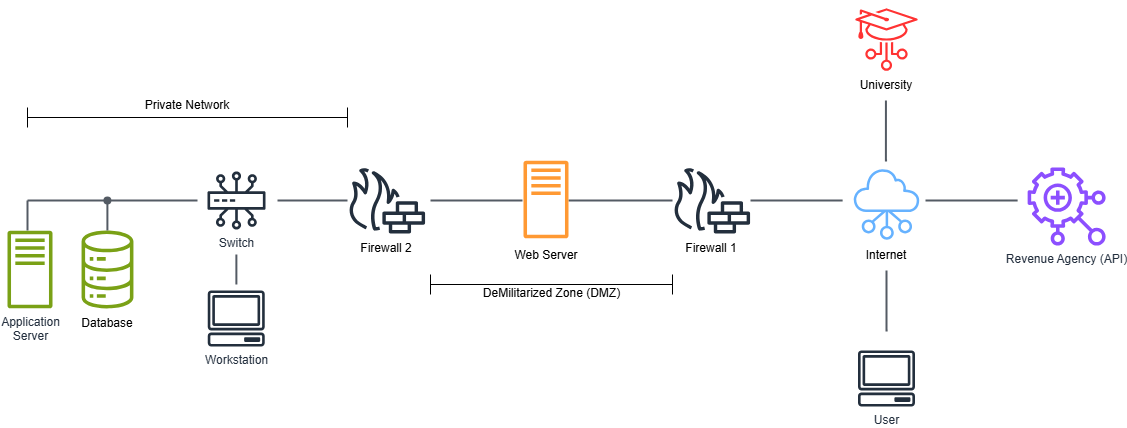
\includegraphics[width=15cm]{images/architectural design/overview.png}
    \caption{Overview of the S\&C system}
\end{figure}
This diagram illustrates the platform's entire architecture, highlighting how the components are interconnected and how security is ensured. 
The \textbf{Private Network} is the backbone of the platform. It hosts the \textbf{Application Server}, which runs the system's logic, and the \textbf{Database} where all the data is stored. These components are connected via a switch to a Workstation used for internal administration, such as company registrations.\newline
The \textbf{Demilitarized Zone} (DMZ) contains the Web Server, which handles user requests. 
The DMZ is placed between the two firewalls. This is standard practice to ensure that external users can only access the components within the DMZ (in this case, the Web Server) while maintaining the security of components inside the Private Network.\newline
On the \textbf{Internet}-facing side, the platform interacts with users and integrates with external services, such as the university SSO systems and the Revenue Agency APIs.
\pagebreak
\section{Component view}
\begin{figure}[H]
    \centering
    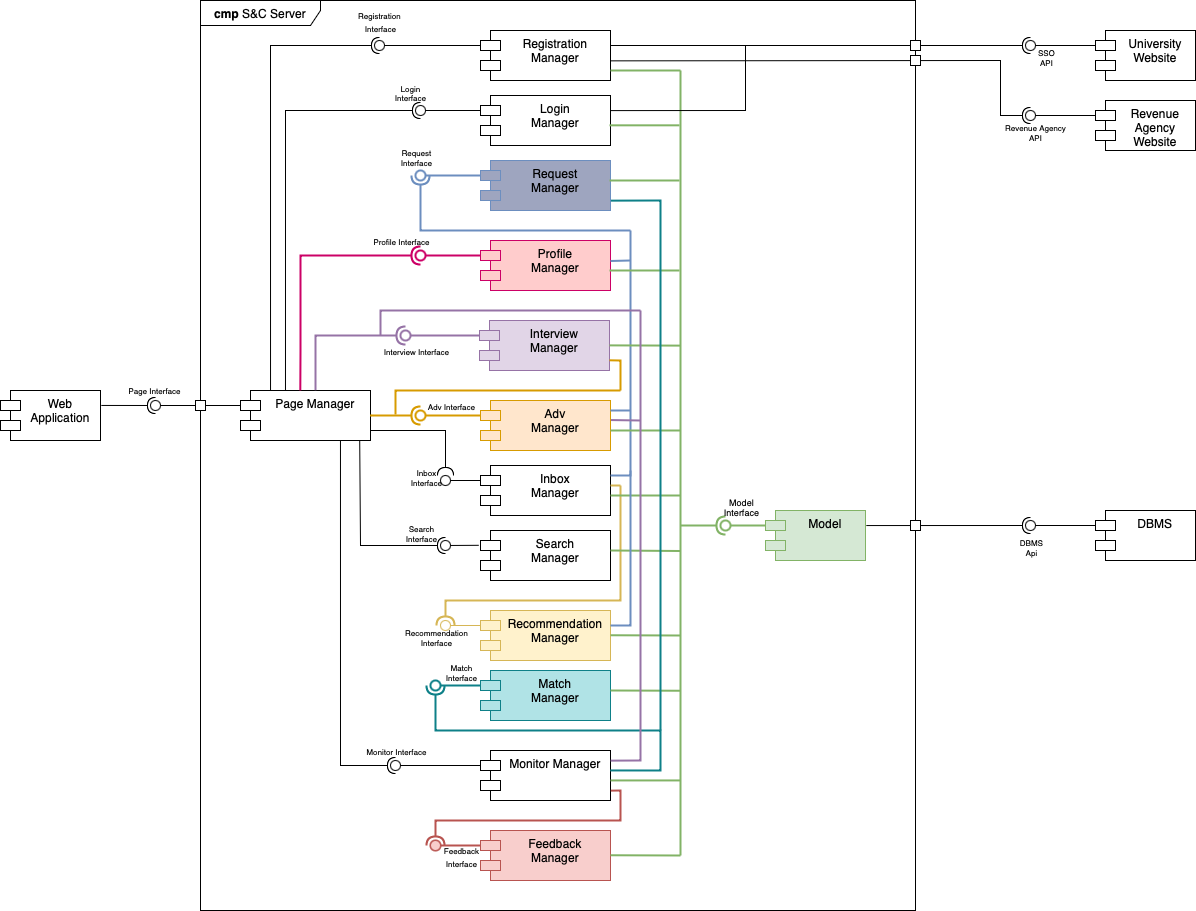
\includegraphics[width=15cm]{images/architectural design/DD-ArchitecturalManager.png}
    \caption{Component view: Low Level Diagram}
    \label{figure:LowLevelDiagram}
\end{figure}
The figure \ref{figure:LowLevelDiagram} represent the S\&C architecture the Server's components:
\begin{itemize}
    \item \textbf{Page Manager:} This component directs the User's requests through the Page Interface to the correct component. It acts like a switch for whole the server.
    
    \item \textbf{Registration Manager:} This component handles new User registration, receiving the request from the Page Manager, and communicating with the university SSO API, if the user is a Student or with the Revenue Agency API, if the user is a Company. This component communicates also with the Users DBMS saving information about the new User.

    \item \textbf{Login Manager:} This component handles the login of an existing User, it communicates with the Users DBMS in order to check the validity of the credentials used by the User.

    \item \textbf{Request Manager:} This component is responsible for managing the Request of a Company to contact a Student and vice versa. If a Request is accepted the creation of a Match will be triggered.

    \item \textbf{Profile Manager:} This component loads the Profile Page of both Students and Companies by communicating with the Users DBMS. This component, also, communicates with Request Manager in order to create a Request in case a visitor of the profile wants to contact the owner.

    \item \textbf{Interview Manager:} This component handles the request from the Adv Manager regarding the creation of a new Interview Form by the Users (C) and manages the interview requests.

    \item \textbf{Adv Manager:} This component handles the requests regarding the Adv Page: it loads the page by communicating with the DBMS, uses Request's interface to allow User (S) to send Requests to the Company proposing the Adv, and allow User (C) to create the Interview form thanks to Interview Manager's interface.

    \item \textbf{Inbox Manager:} This component handles the requests by the Page Manager regarding the Inbox Page that is loaded communicating with the DBMS. Also, it communicates with Request and Recommendation Manager to allow User to answer an internship request and contact the Users suggested in the Recommendation.

    \item \textbf{Search Manager:} This component handles the Page Manager's request about Search Page, and collects the results of the research made by the User by communicating with the DBMS.

    \item \textbf{Recommendation Manager:} This component handles the creation of recommendations using the data in the DBMS, uses the interface of Request Manager to let Users contact the suggestions made in the recommendation, and supplies to the Inbox Manager an interface to load the recommendation page.

    \item \textbf{Match Manager:} This component handles the request from the Monitor Manager regarding the information about a Match state by communicating with the DBMS.

    \item \textbf{Monitor Manager:} This component handles the requests by the Page Manager regarding the Monitor Page that is loaded communicating with the DBMS, Match Manager and Interview Manager. Also, it communicates with Feedback Manager in order to allow User to leave a feedback in certain states of the Match.

    \item \textbf{Feedback Manager:} This component handles the request from the Monitor Manager regarding the creation of a new Feedback from the Users.

    \item \textbf{Model:} This component handles the communication with the DBMS to fulfill all the requests of the other components about saving, deleting, getting or modifying data.
    
\end{itemize}
\pagebreak
\section{Deployment view}
Here follows the \textbf{Deployment Diagram} of the S\&C system.
\begin{figure}[H]
    \centering
    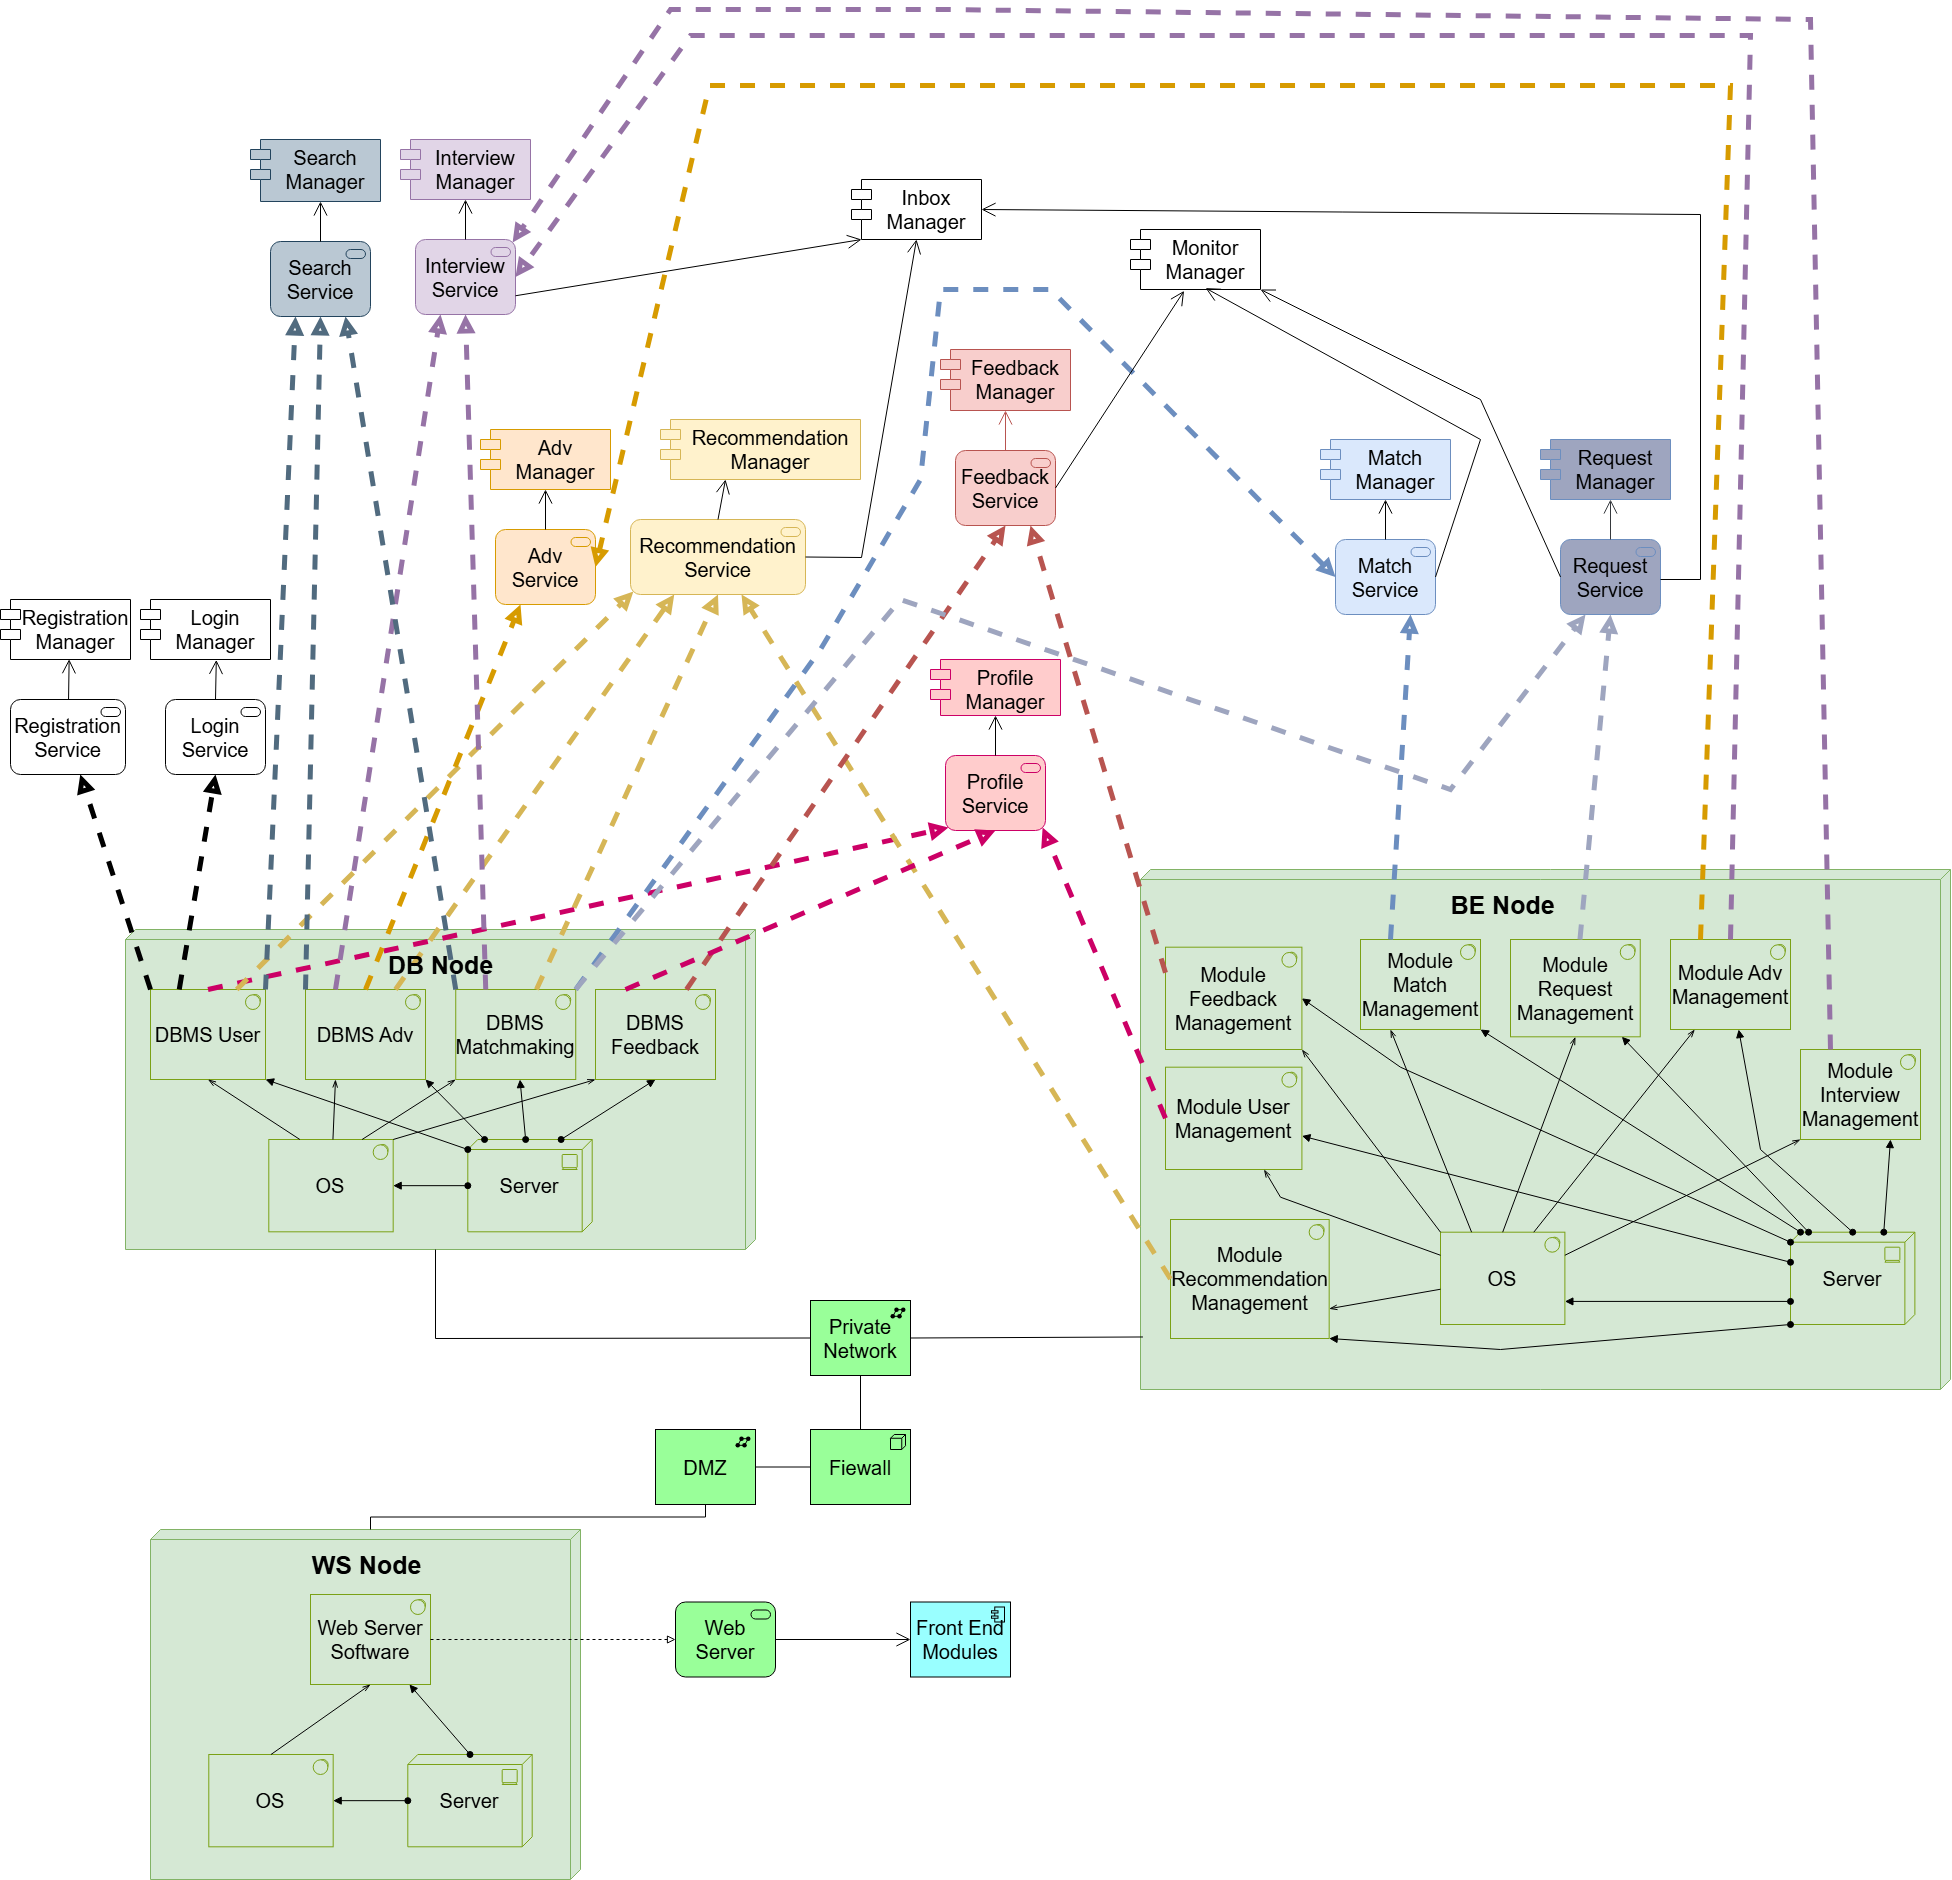
\includegraphics[width=15cm]{images/architectural design/deployment/DD-deploymentdiagram2.drawio.png}
    \caption{Deployment Diagram}
\end{figure}
This is an overview of the whole diagram, each node and module is going to be explained in detail with a zoomed image.
\subsection{Architecture nodes}
\begin{figure}[H]
    \centering
    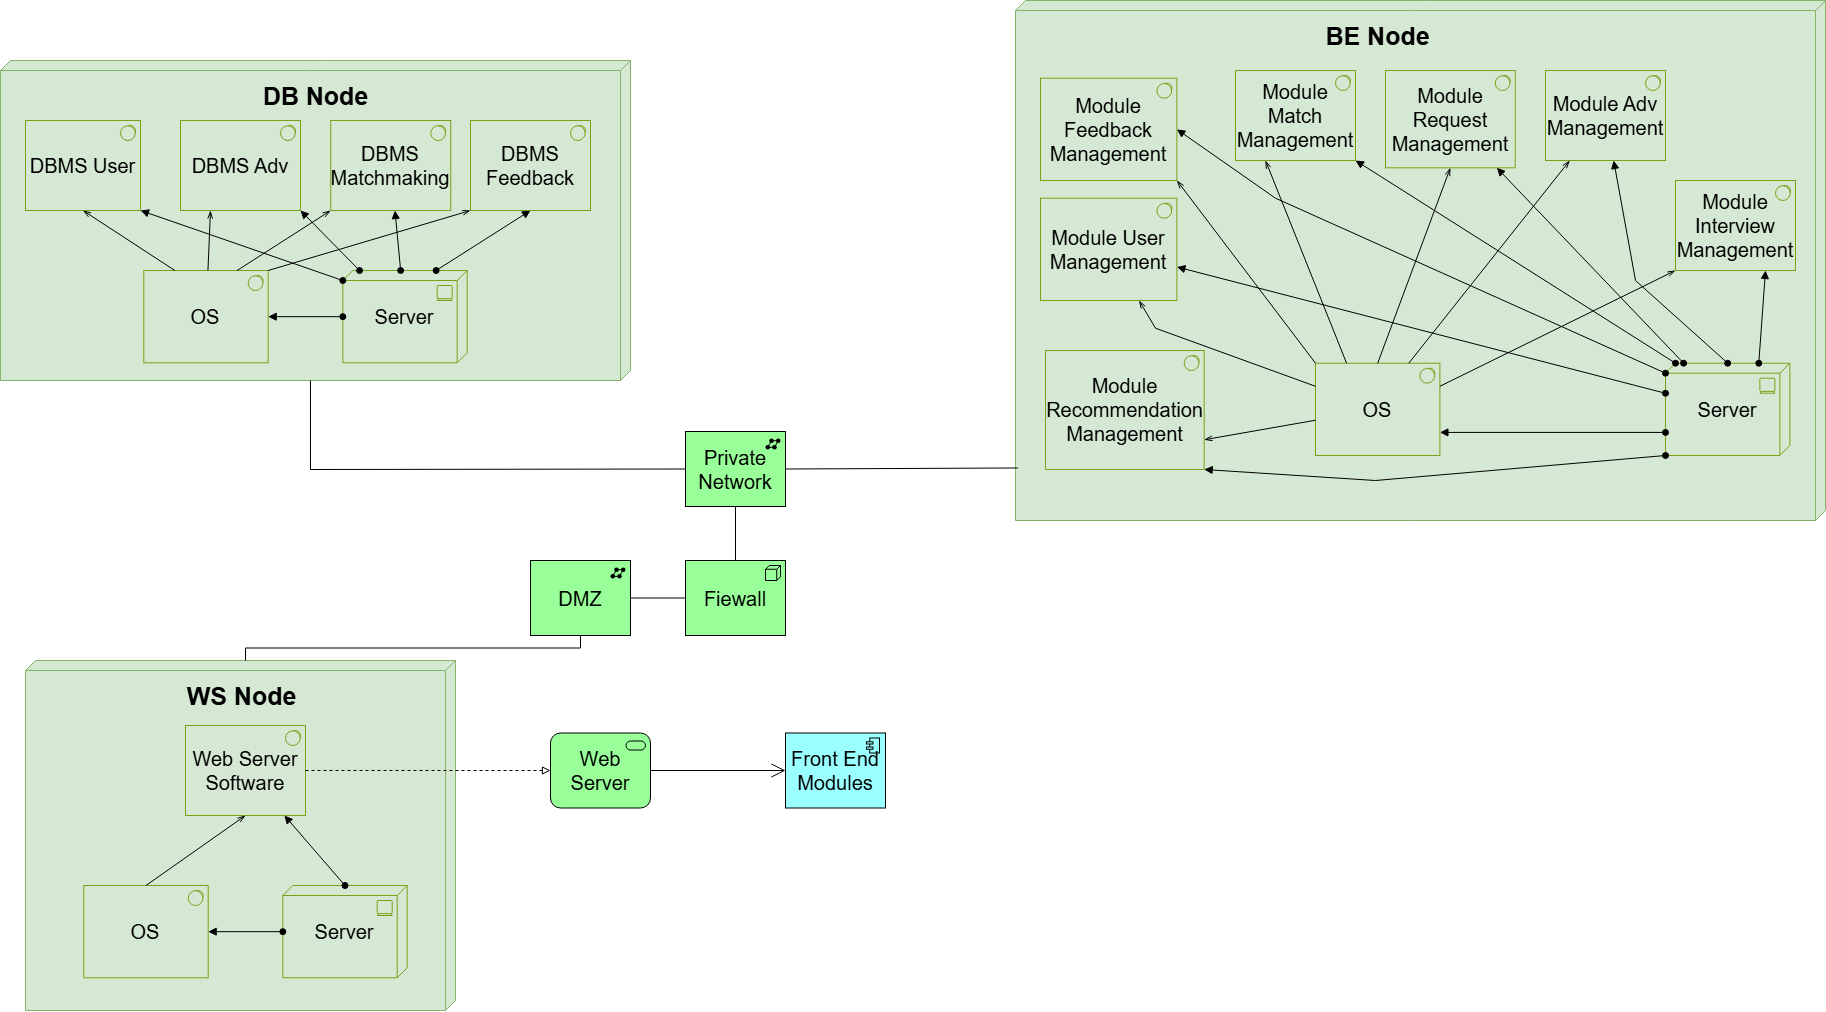
\includegraphics[width=15cm]{images/architectural design/deployment/depl-rete.drawio (1).png}
    \caption{Architecture nodes in Deployment Diagram}
\end{figure}
This is the architecture shown in the Overview Chapter, with the modules and components shown.
\subsubsection{Database Node}
\begin{figure}[H]
    \centering
    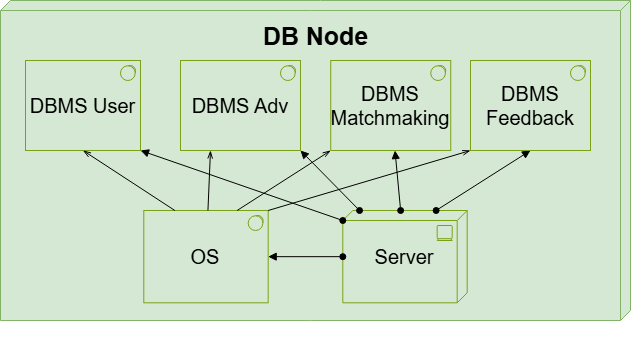
\includegraphics[width=15cm]{images/architectural design/deployment/depl-dbnode.drawio.png}
    \caption{Database Node in Deployment Diagram}
\end{figure}
This node is designed to centralise database management, it divides responsibilities across modules:
\begin{itemize}
    \item \textbf{User}: the DBs contain the information of both kinds of users, students, and companies.
    \item \textbf{Adv}: it organises the data of each internship advertisement, is related to the Company DB via external key.
    \item \textbf{Matchmaking}: it collects data about the matchmaking process: request messages, interview requests, matches' status.
    \item \textbf{Feedback}: feedback of companies and students is collected and connected to the respective user via external key.
\end{itemize}
The Operative System (OS) provides the base system for managing hardware and software resources on the DB Node and ensures the proper execution of database management systems and server processes. The Server facilitates communication between the DB Node and components.
\subsubsection{Back-End Node}
\begin{figure}[H]
    \centering
    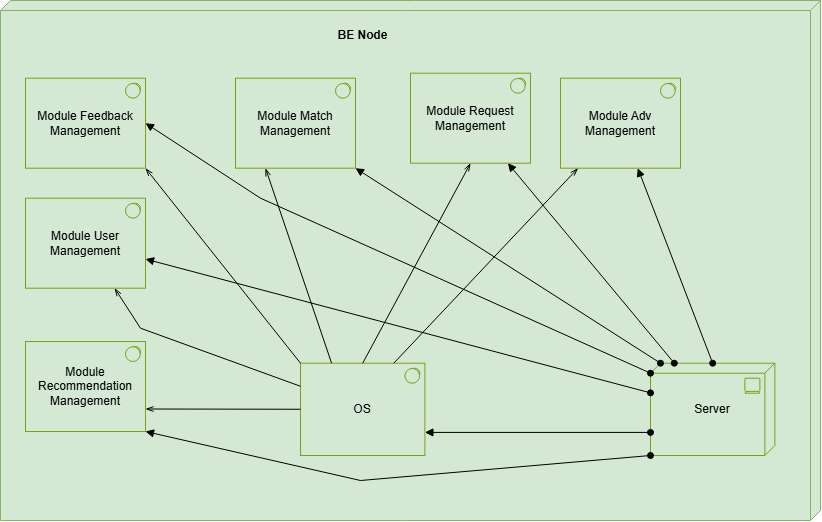
\includegraphics[width=15cm]{images/architectural design/deployment/depl-be.drawio.png}
    \caption{Back-End Node in Deployment Diagram}
\end{figure}
This node contains the business logic of the system, every module present runs specific functionalities related to the components, each module is seen in detail with the respective components and services. 
\subsection{Components and services}
\subsubsection{Sign up and Login}
\begin{figure}[H]
    \centering
    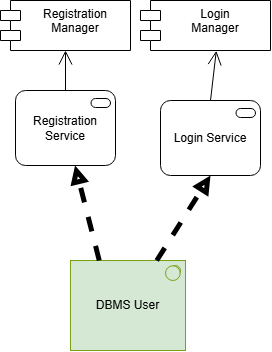
\includegraphics[width=0.25\linewidth]{images/architectural design/deployment/depl-login-signup.drawio.png}
    \caption{Deployment Diagram: Login and Sign up}
\end{figure}
Users sign up and logins are managed through database's query, so their services relies entirely on the User DBMS.
\subsubsection{Profile Management}
\begin{figure}[H]
    \centering
    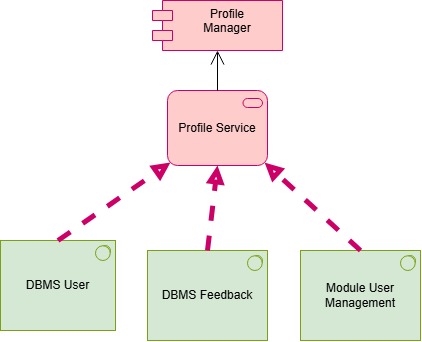
\includegraphics[width=0.40\linewidth]{images/architectural design/deployment/depl-profile.drawio.png}
    \caption{Deployment Diagram: Profile Management}
\end{figure}
Users' data is stored inside the DB so profiles are managed through queries to the DB and the functions inside the \textbf{Module Profile Manager}.

\subsubsection{ADV Management}
\begin{figure}[H]
    \centering
    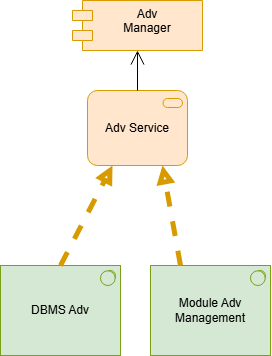
\includegraphics[width=0.25\linewidth]{images/architectural design/deployment/deply-adv.drawio.png}
    \caption{Deployment Diagram: ADV Management}
\end{figure}
ADV's data is stored inside the DB, while the functions to manage them are found in the \textbf{Manage ADV Module}.

\subsubsection{Interview Management}
\begin{figure}[H]
    \centering
    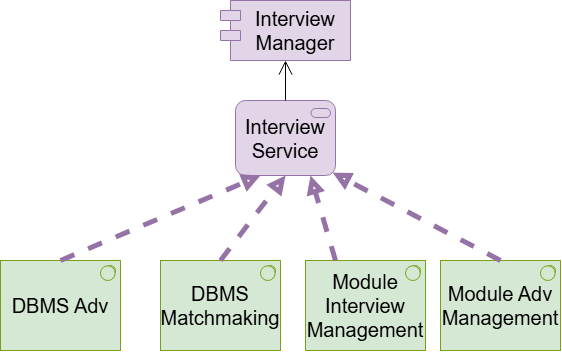
\includegraphics[width=0.45\linewidth]{images/architectural design/deployment/depl-inter.drawio.png}
    \caption{Deployment Diagram: Interview Management}
\end{figure}
Interview Manager handles interview forms and interview requests. Interview forms are stored in the \textbf{Adv DBMS} and managed by both \textbf{Module Adv Management} and \textbf{Module Interview Manager}, while interview requests are stored inside the \textbf{Matchmaking DBMS} and managed by the \textbf{Module Interview Management}.

\subsubsection{Search Management}
\begin{figure}[H]
    \centering
    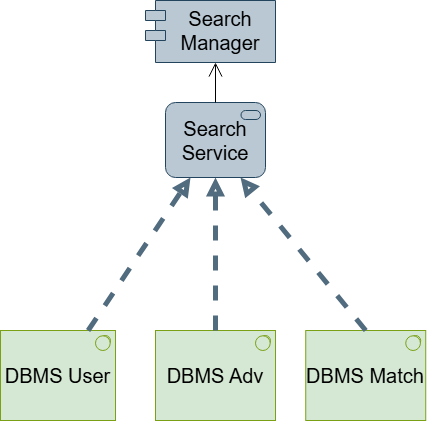
\includegraphics[width=0.25\linewidth]{images/architectural design/deployment/depl-search.drawio (1).png}
    \caption{Deployment Diagram: Search Management}
\end{figure}
User searches rely on the Users DB and on the ADV, they are managed through queries. Also, the fields inserted by the students are stored inside the correspondent DB (in the User DBMS) in order to make proper recommendations. The search results cannot be already matched with the user searching, so the results are checked with the matches inside the DB.

\subsubsection{Recommendation Management}
\begin{figure}[H]
    \centering
    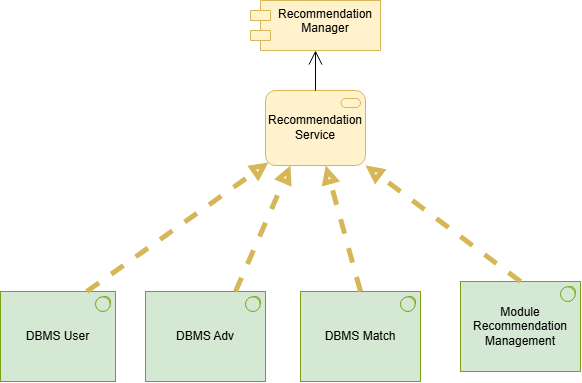
\includegraphics[width=0.45\linewidth]{images/architectural design/deployment/depl-recc.drawio.png}
    \caption{Deployment Diagram: Recommendation Management}
\end{figure}
Recommendations are based on Users and ADVs, so they are based on the data in the DBs and managed through the functions in the \textbf{Recommendation Manager}. They can also queries the Matchmaking DBMS to make sure that the recommended profiles are not already matched. 

\subsubsection{Match Management}
\begin{figure}[H]
    \centering
    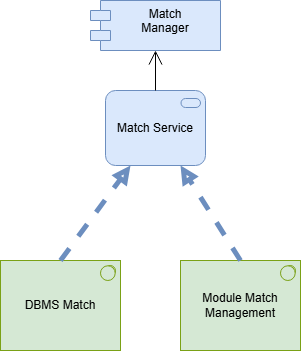
\includegraphics[width=0.25\linewidth]{images/architectural design/deployment/depl-match.drawio.png}
    \caption{Deployment Diagram: Match Management}
\end{figure}
Matches are stored in the DB and are managed through the functions of \textbf{Module Match Management}.

\subsubsection{Feedback Management}
\begin{figure}[H]
    \centering
    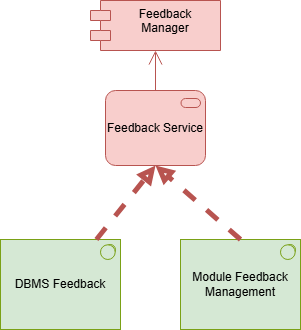
\includegraphics[width=0.25\linewidth]{images/architectural design/deployment/depl-feed.drawio.png}
    \caption{Deployment Diagram: Feedback Management}
\end{figure}
Feedbacks are stored inside the DB and are managed through the \textbf{Module Feedback Management}.

\subsubsection{Monitor and Inbox Management}
\begin{figure}[H]
    \centering
    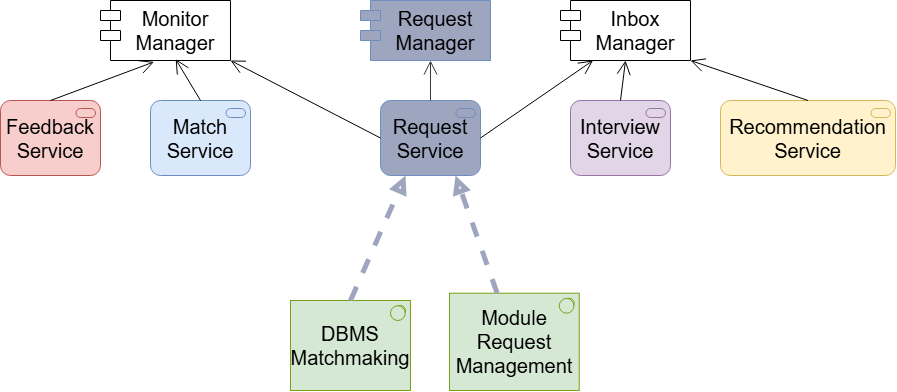
\includegraphics[width=0.65\linewidth]{images/architectural design/deployment/depl-requ.drawio.png}
    \caption{Deployment Diagram: Monitor and Inbox Management}
\end{figure}
The Monitor Section shows the user's matches, and it is where users can leave feedbacks, so it is based on the \textbf{Match Service}, the \textbf{Request Service}, and the \textbf{Feedback Service}.
The Inbox Section shows match and interview requests, and recommendations sent to the user, so it is based on the \textbf{Request Service} that is managed through the \textbf{Module Request Manager}, the \textbf{Recommendation Service}, and the \textbf{Interview Serivce}. 
\section{Runtime view}
\begin{figure}[H]
\textbf{Student Sign up}\newline\newline
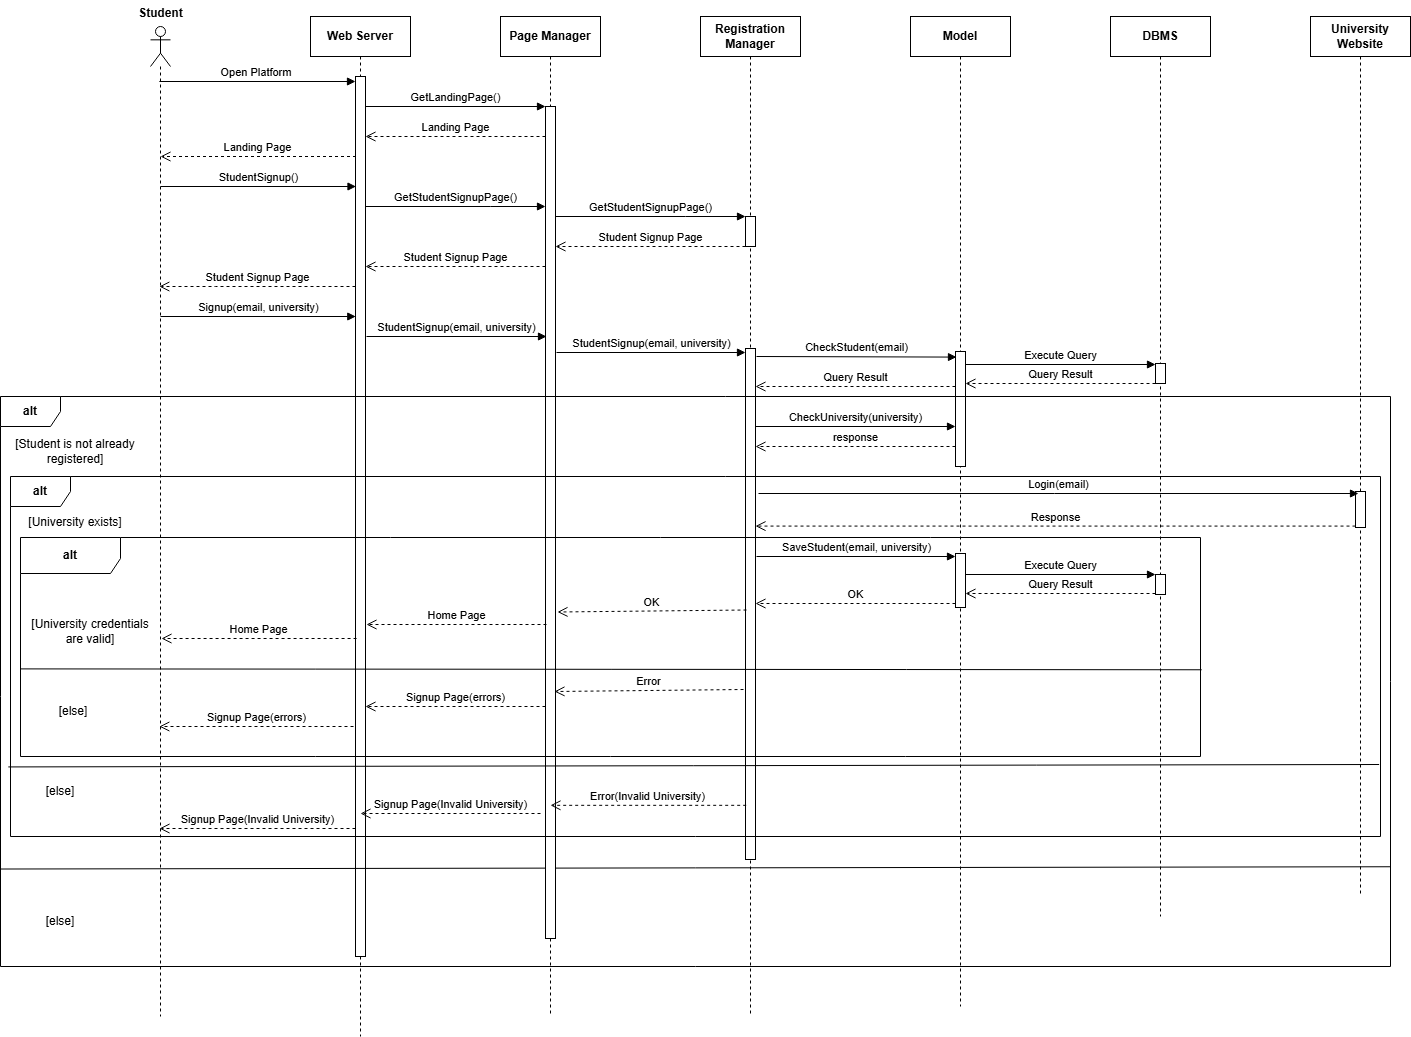
\includegraphics[width=15cm]{images/architectural design/runtime/DD-UC1.drawio (1).png}
    \caption{SD: Student Sign up}
\end{figure}

\begin{figure}[H]
\textbf{Student Login}\newline\newline
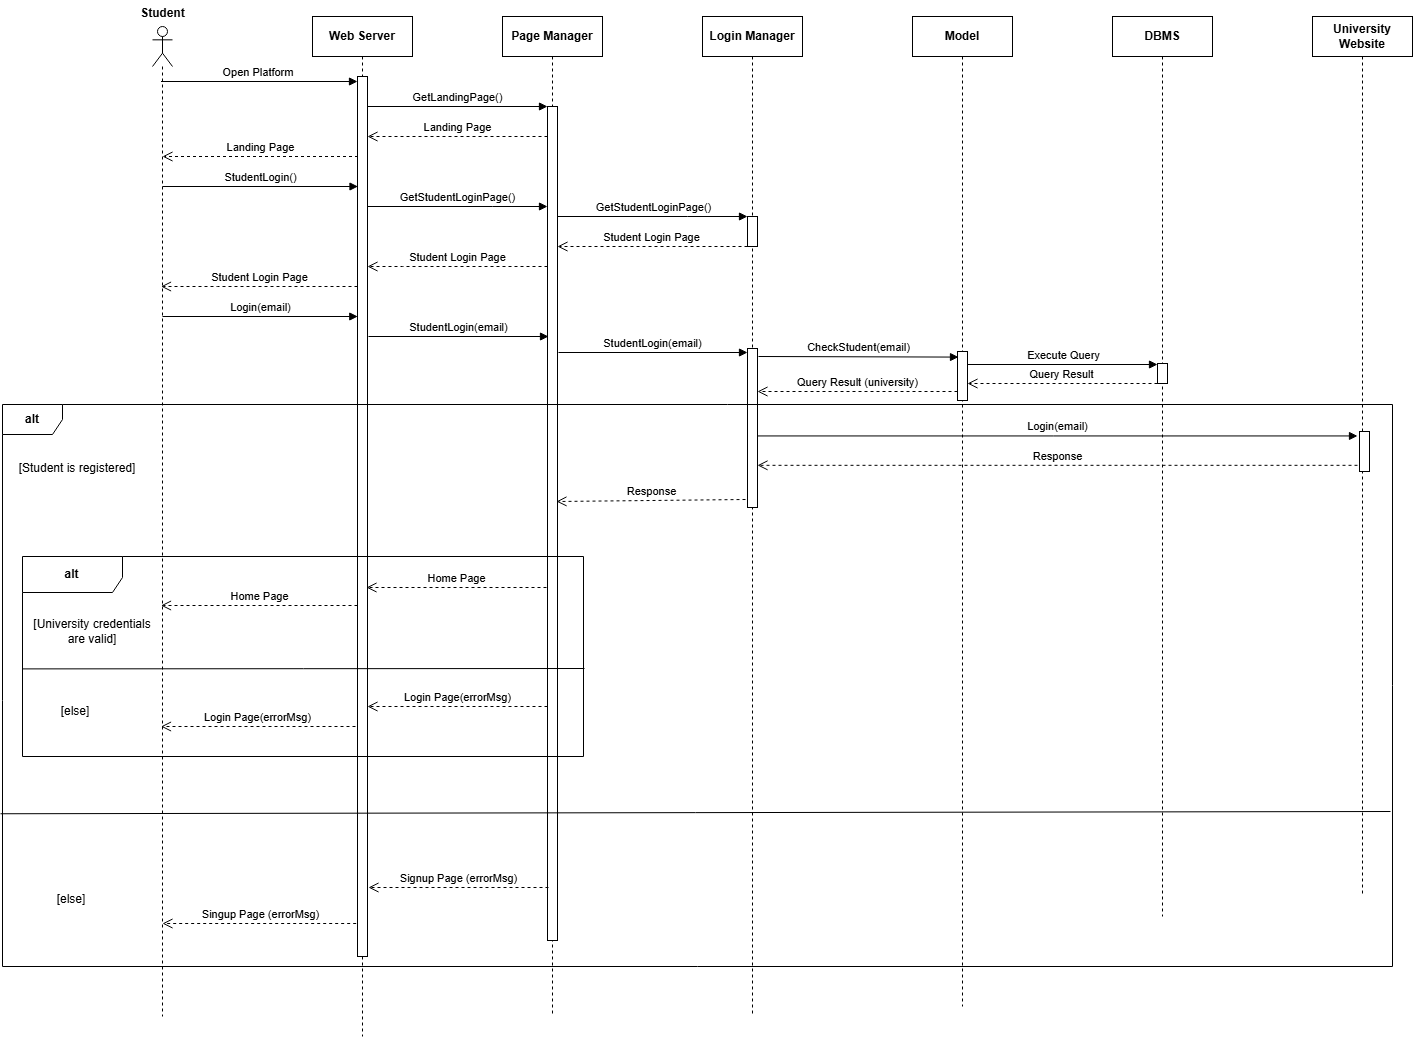
\includegraphics[width=15cm]{images/architectural design/runtime/DD-UC2.drawio.png}
    \caption{SD: Student Login}
\end{figure}

\begin{figure}[H]
\textbf{Company Sign up}\newline\newline
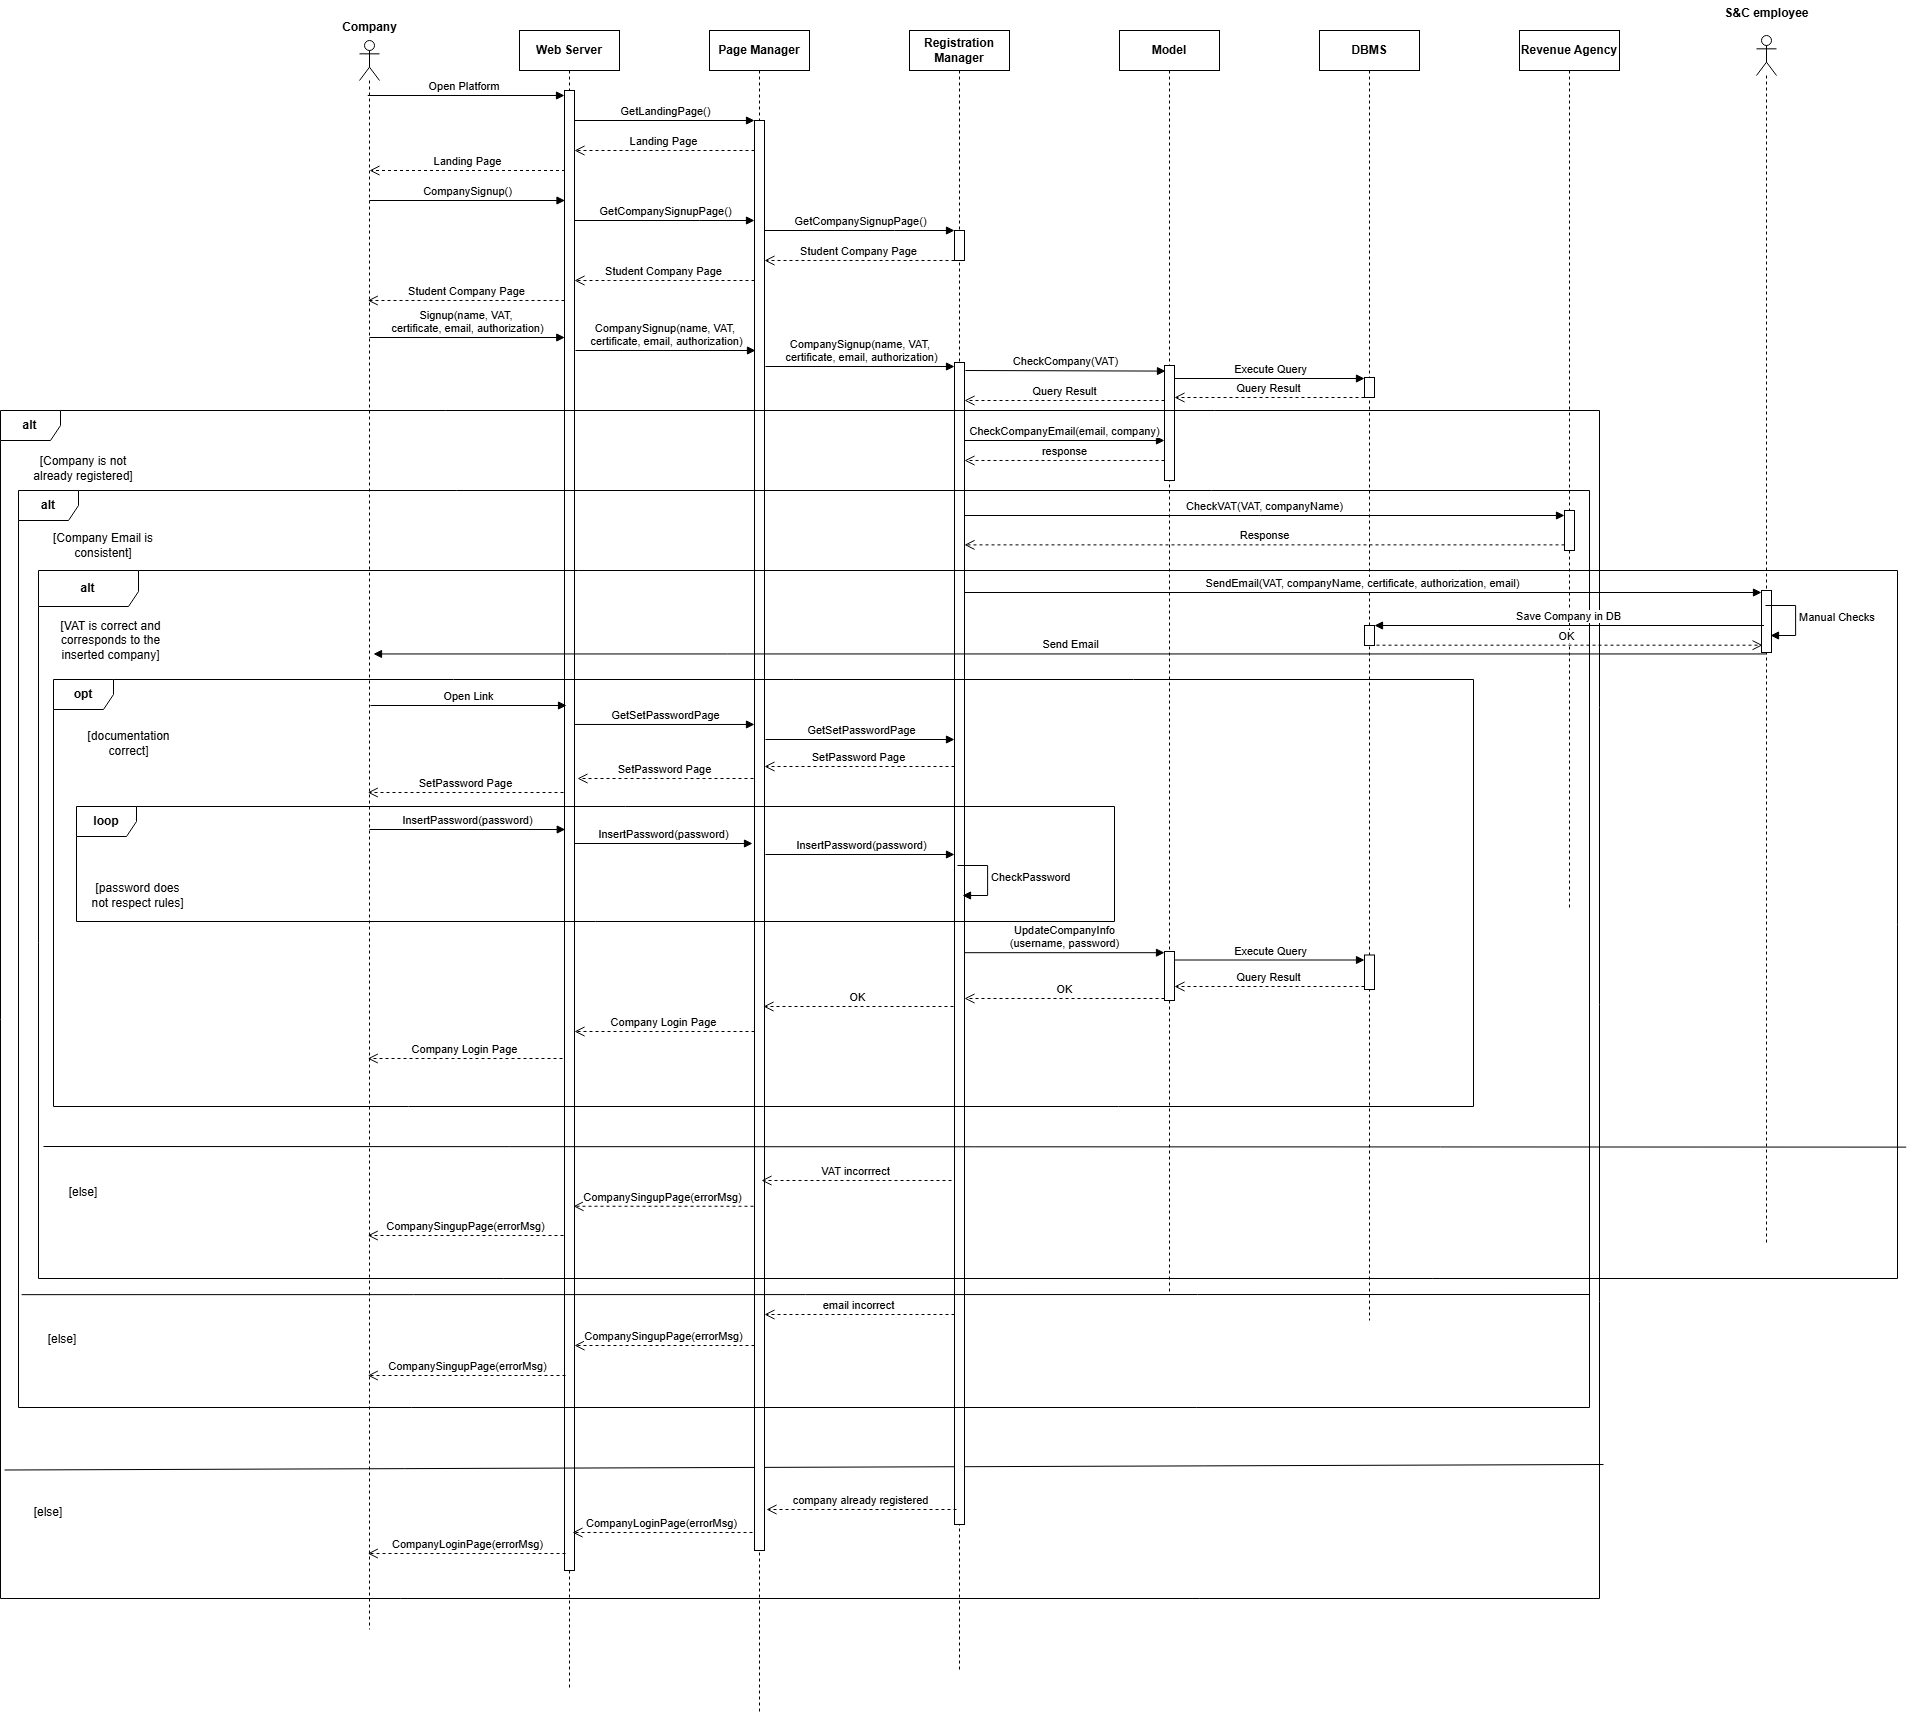
\includegraphics[width=15cm]{images/architectural design/runtime/DD-UC3.drawio.png}
    \caption{SD: Company Sign up}
\end{figure}

\begin{figure}[H]
\textbf{Company Login}\newline\newline
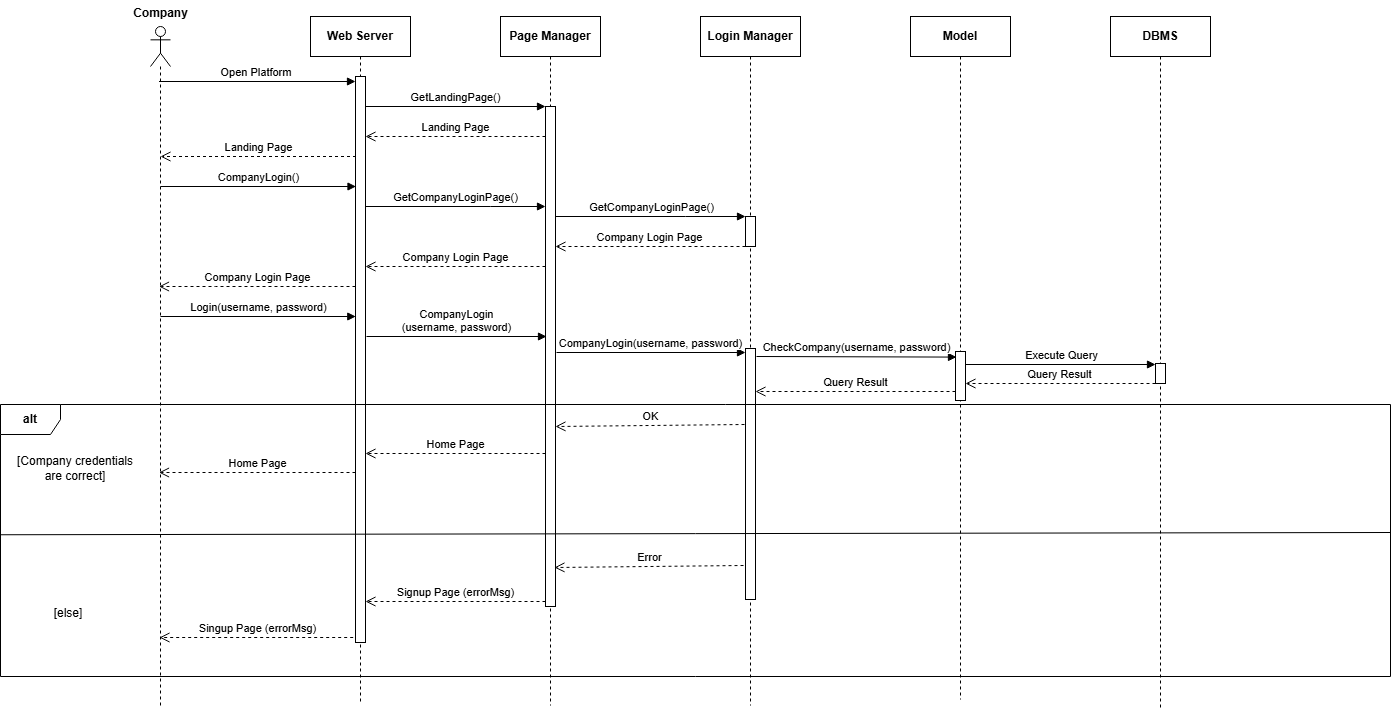
\includegraphics[width=15cm]{images/architectural design/runtime/DD-UC4.drawio.png}
    \caption{SD: Company Login}
\end{figure}

\begin{figure}[H]
\textbf{Upload Student CV}\newline\newline
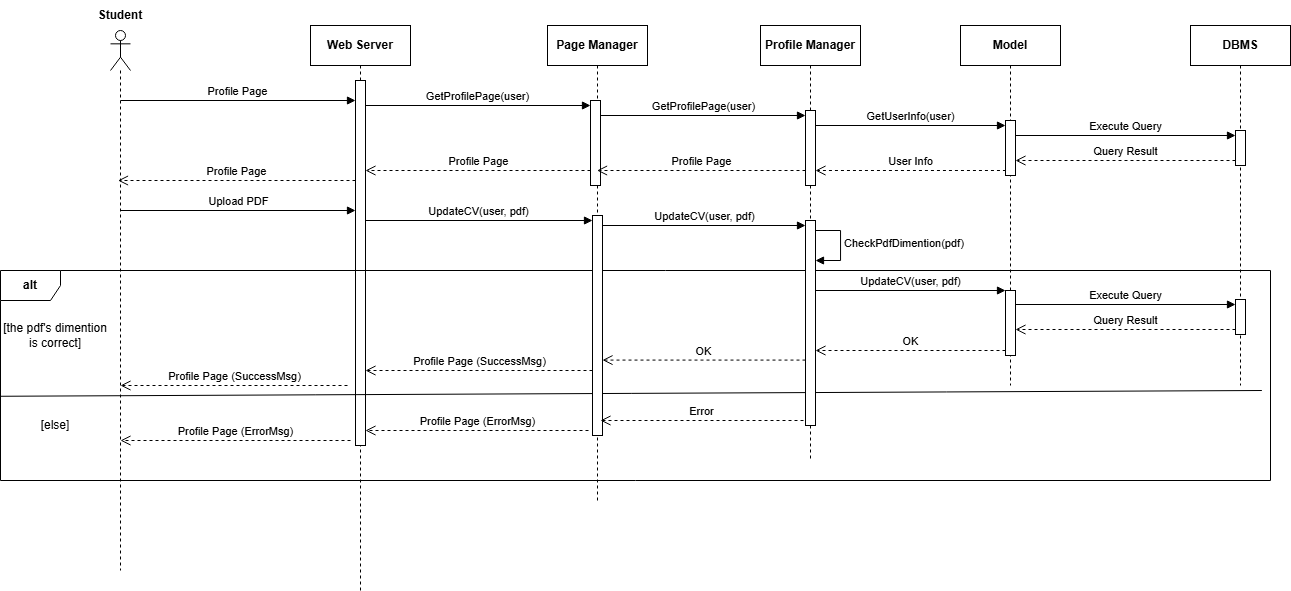
\includegraphics[width=15cm]{images/architectural design/runtime/DD-UC5.drawio.png}
    \caption{SD: Upload Student CV}
\end{figure}

\begin{figure}[H]
\textbf{Add new competence}\newline\newline
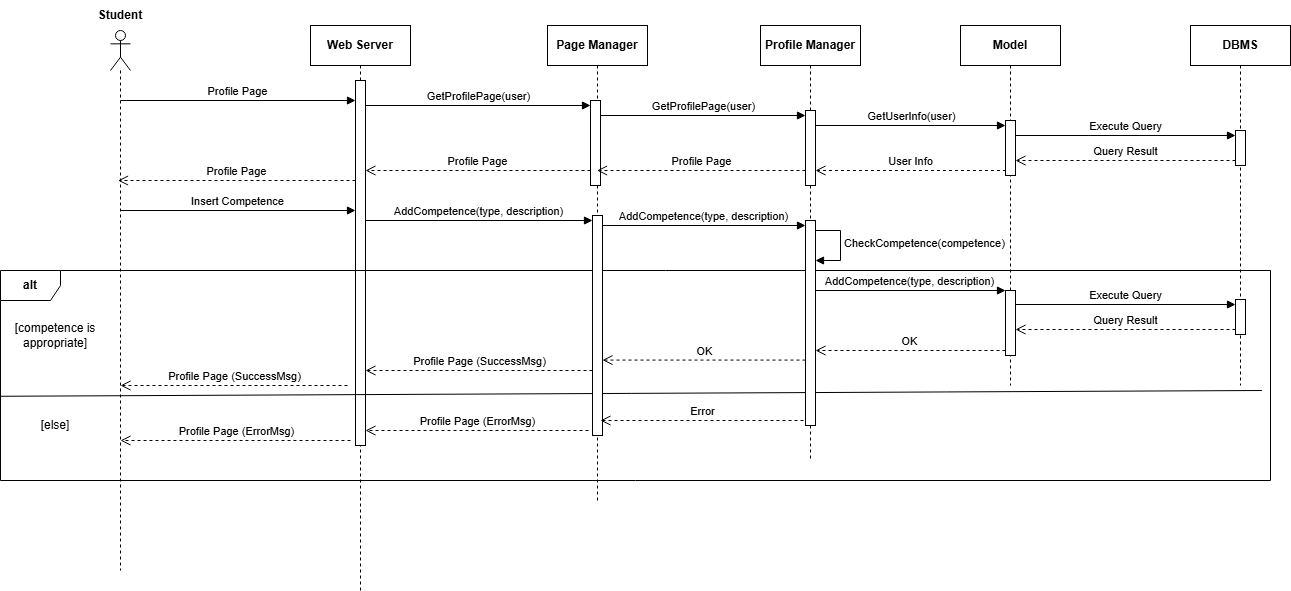
\includegraphics[width=15cm]{images/architectural design/runtime/DD-UC6.drawio.png}
    \caption{SD: Add new competence}
\end{figure}

\begin{figure}[H]
\textbf{Edit competence}\newline\newline
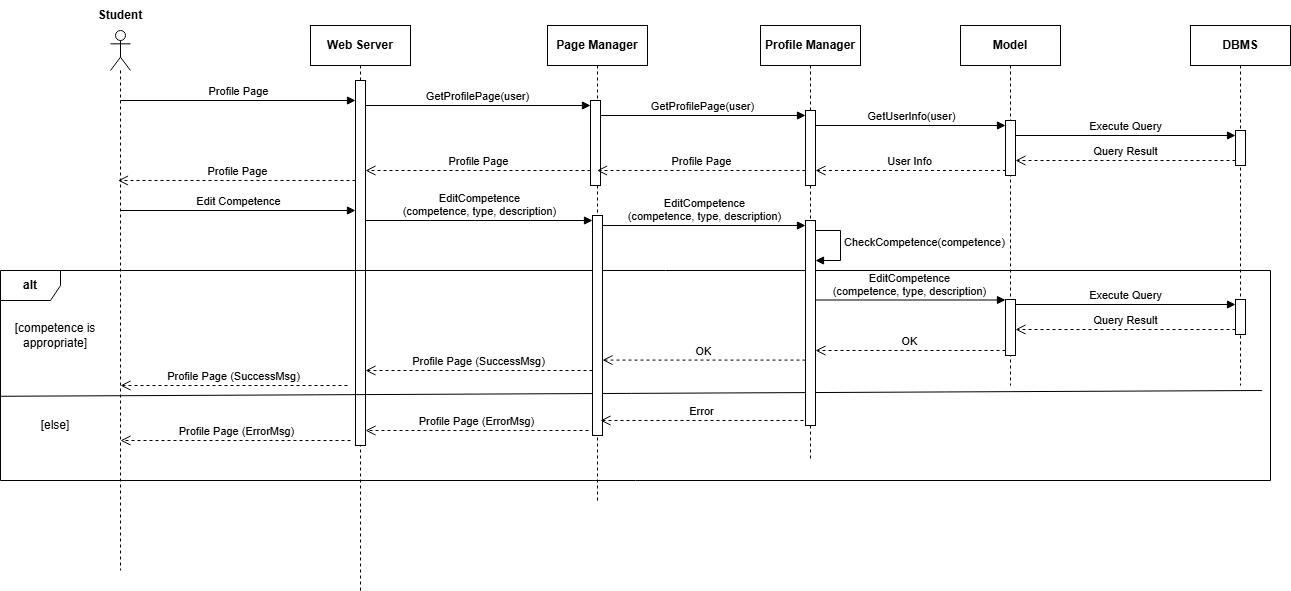
\includegraphics[width=15cm]{images/architectural design/runtime/DD-UC7.drawio.png}
    \caption{SD: Edit competence}
\end{figure}

\begin{figure}[H]
\textbf{Create New ADV}\newline\newline
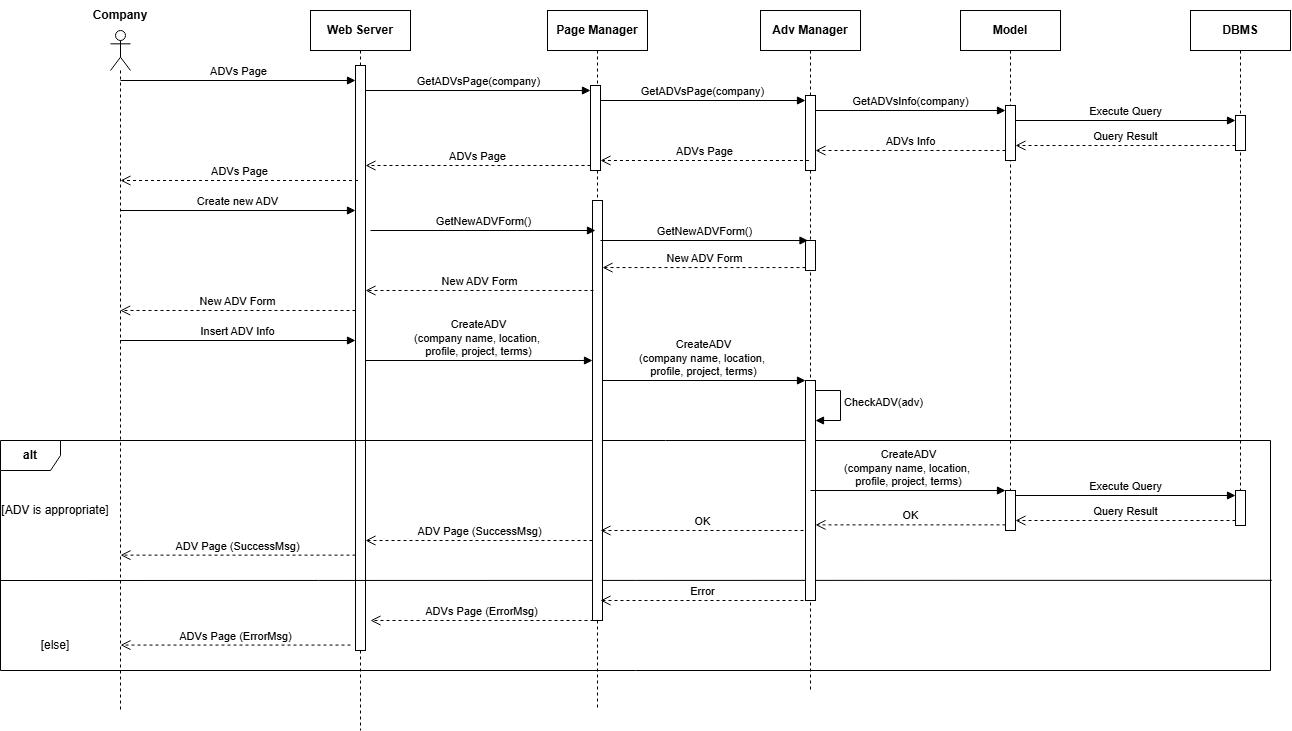
\includegraphics[width=15cm]{images/architectural design/runtime/DD-UC8.drawio (1).png}
    \caption{SD: Create New ADV}
\end{figure}

\begin{figure}[H]
\textbf{Edit ADV}\newline\newline
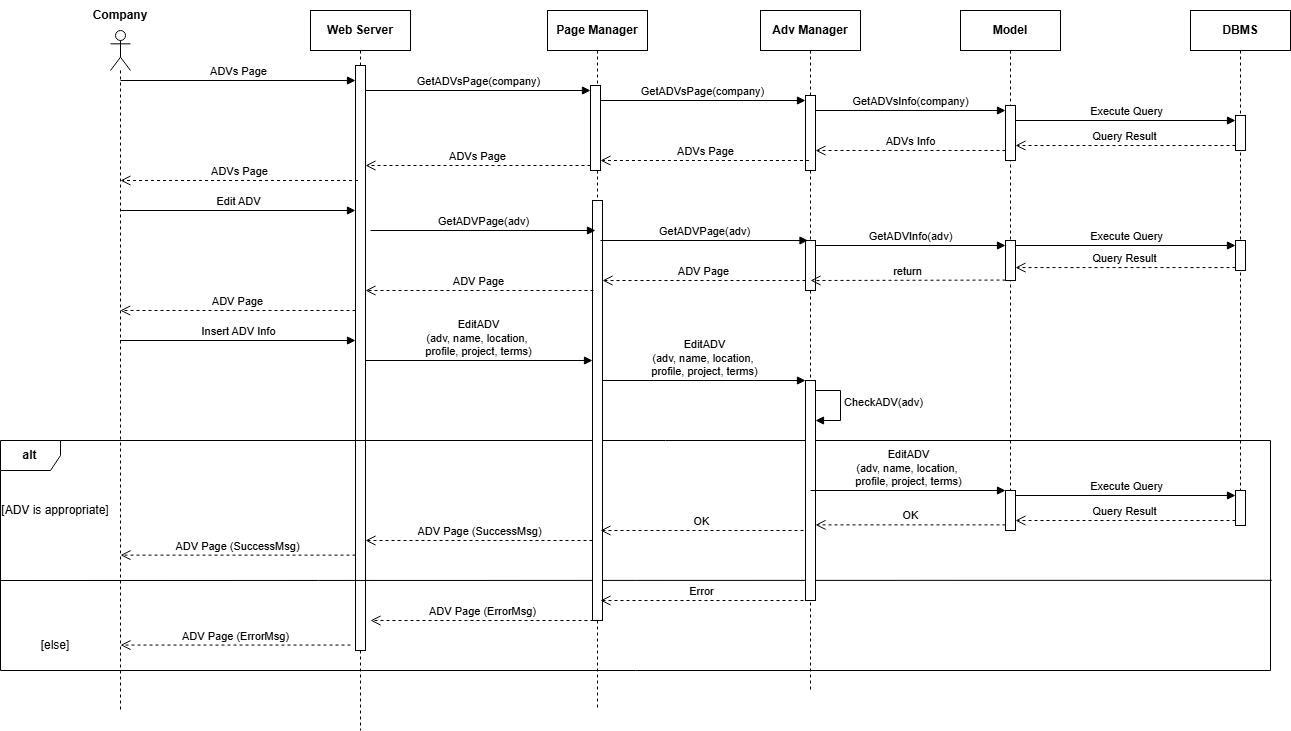
\includegraphics[width=15cm]{images/architectural design/runtime/DD-UC9.drawio (1).png}
    \caption{SD: Edit ADV}
\end{figure}

\begin{figure}[H]
\textbf{Delete ADV}\newline\newline
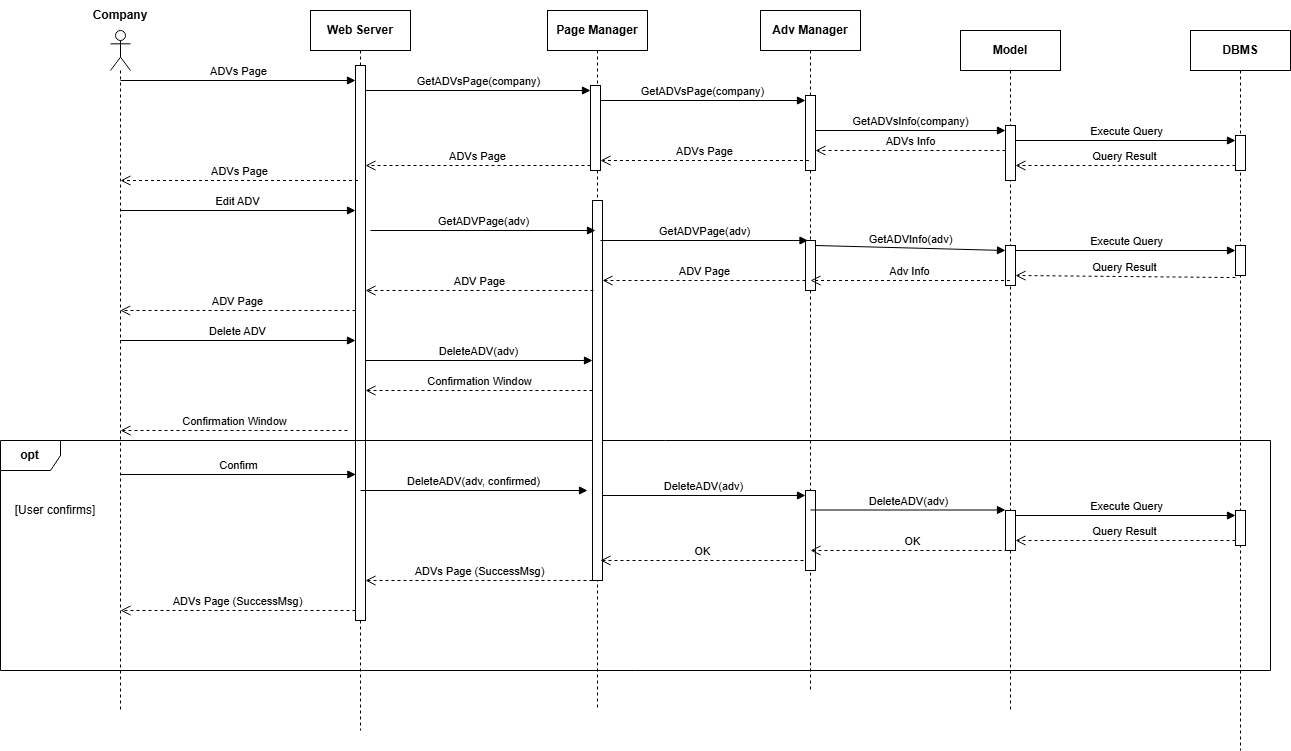
\includegraphics[width=15cm]{images/architectural design/runtime/DD-UC10.drawio (1).png}
    \caption{SD: Delete ADV}
\end{figure}

\begin{figure}[H]
\textbf{Proactive Internship Search}\newline\newline
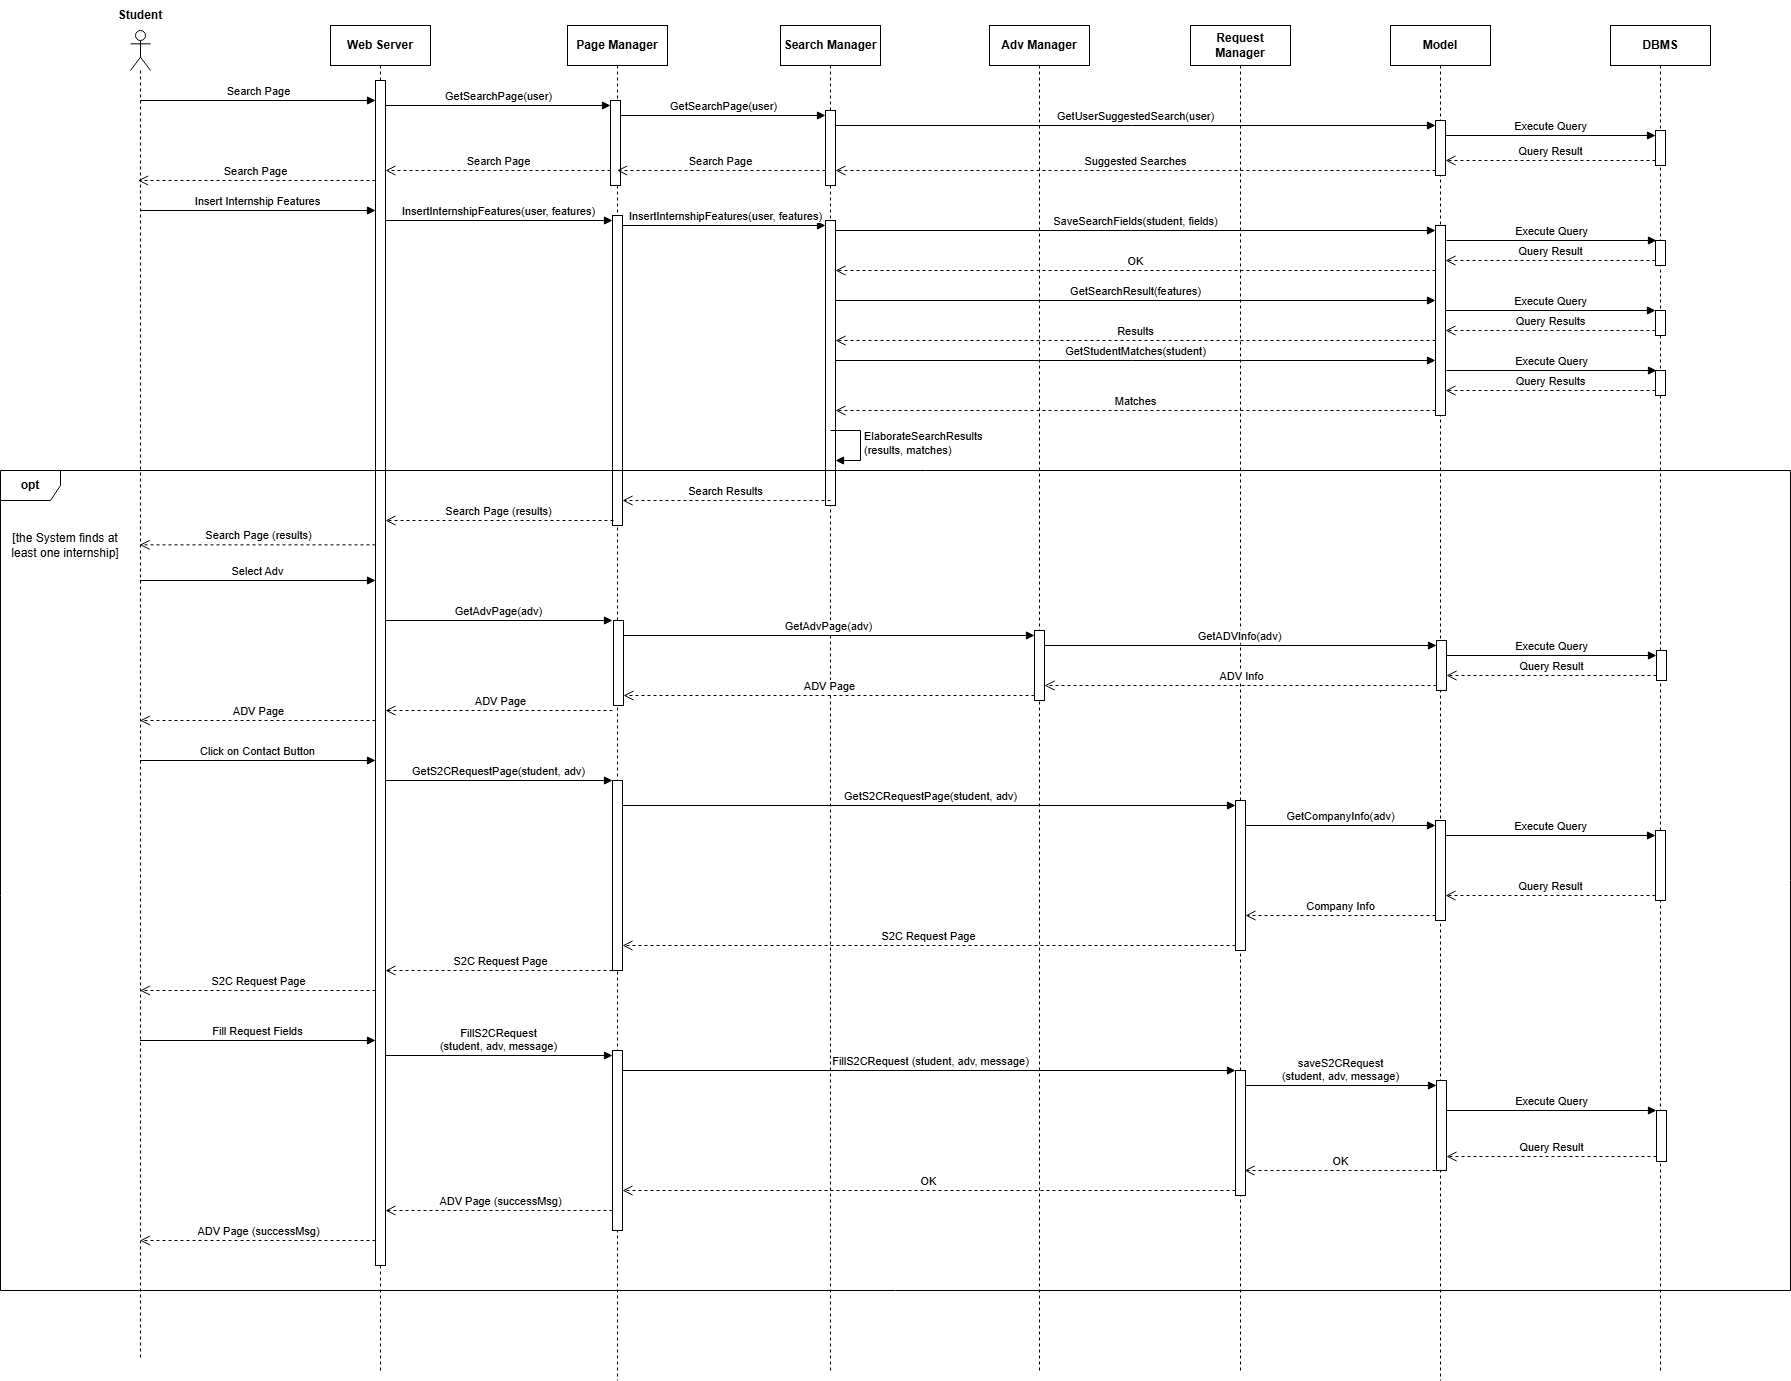
\includegraphics[width=15cm]{images/architectural design/runtime/DD-UC11.drawio.png}
    \caption{SD: Proactive Internship Search}
\end{figure}

\begin{figure}[H]
\textbf{Proactive Candidate Search}\newline\newline
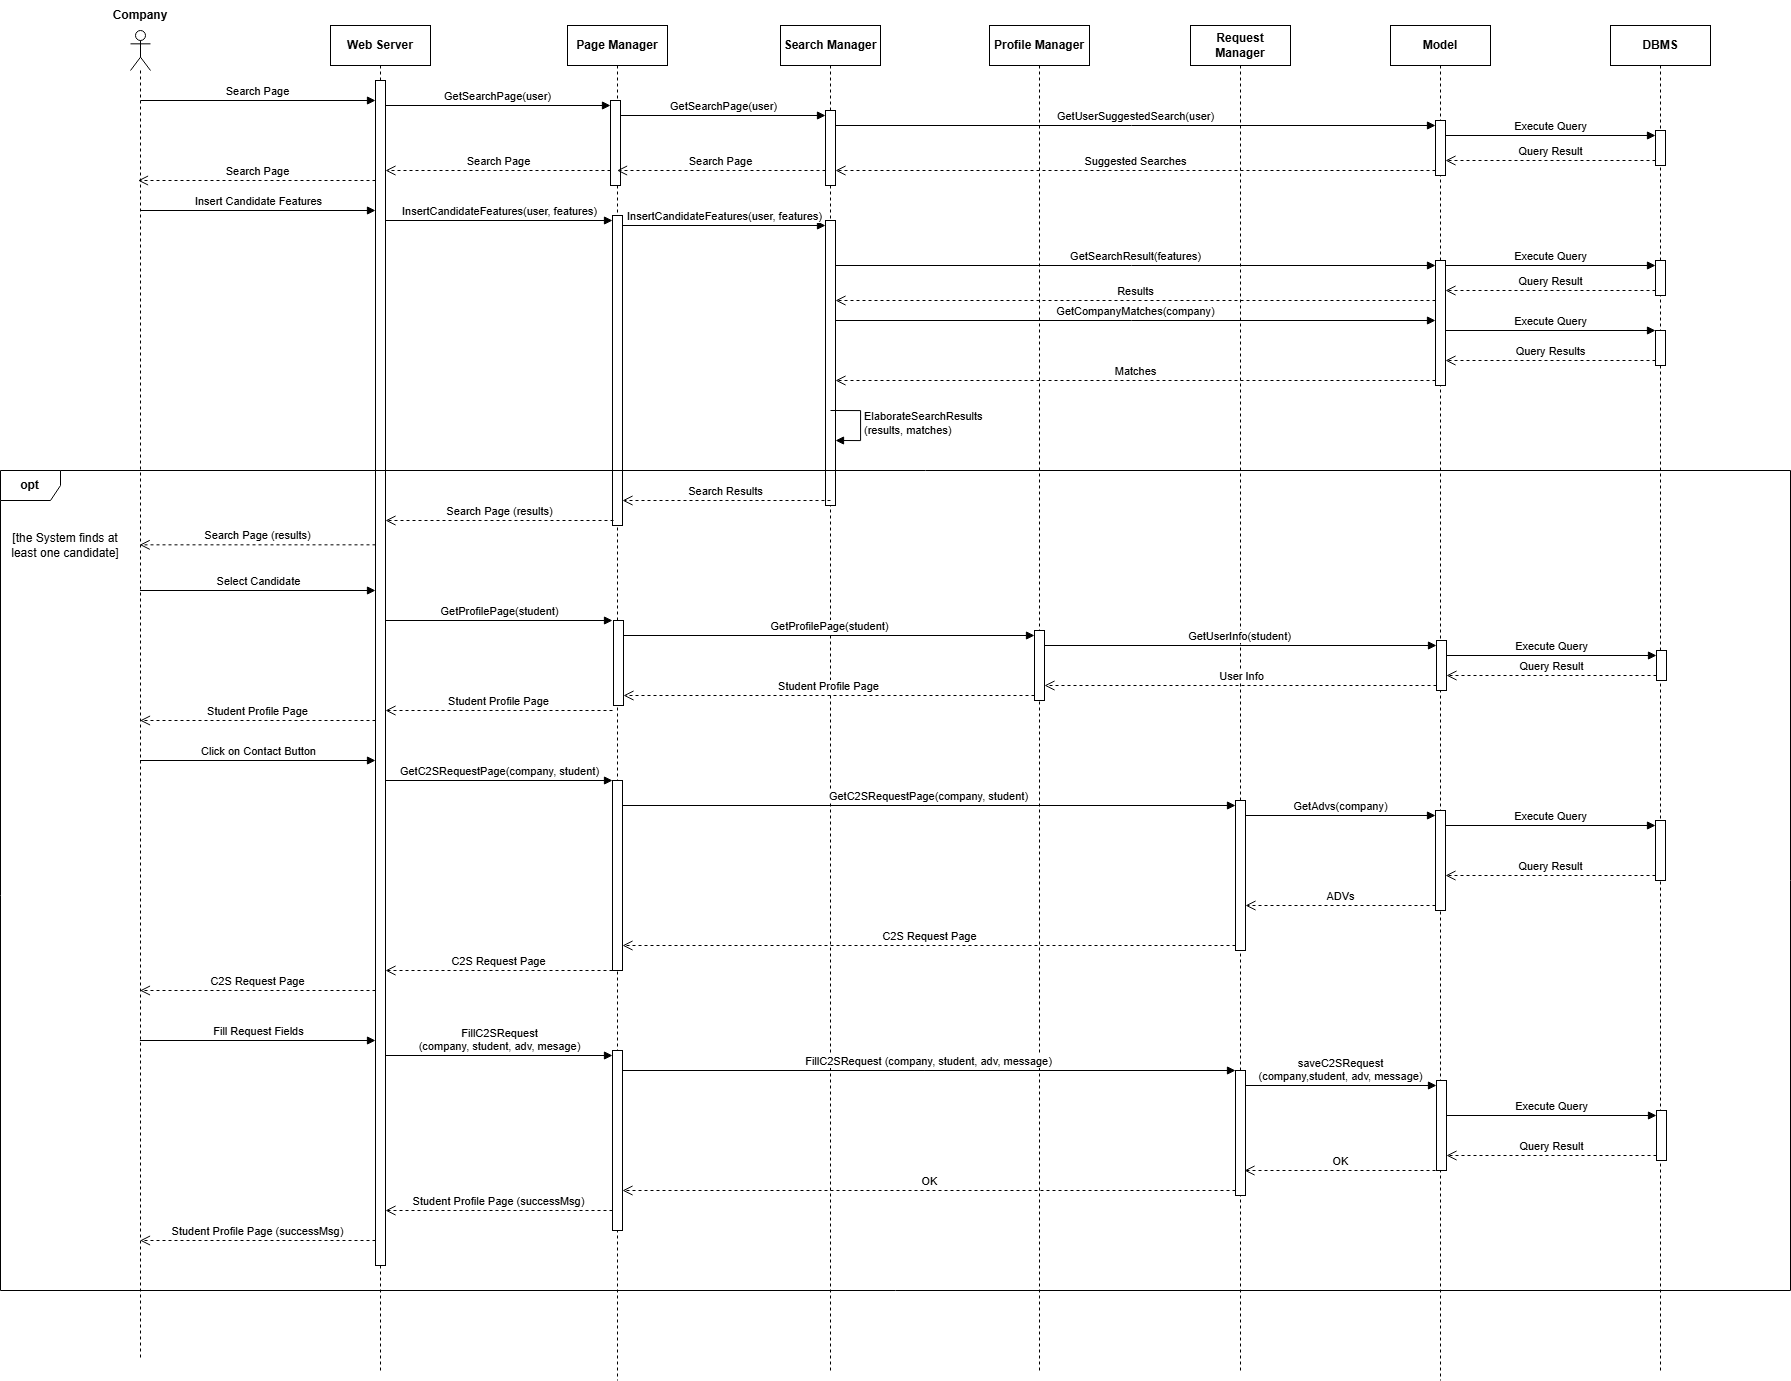
\includegraphics[width=15cm]{images/architectural design/runtime/DD-UC12.drawio.png}
    \caption{SD: Proactive Candidate Search}
\end{figure}

\begin{figure}[H]
\textbf{Recommendation}\newline\newline
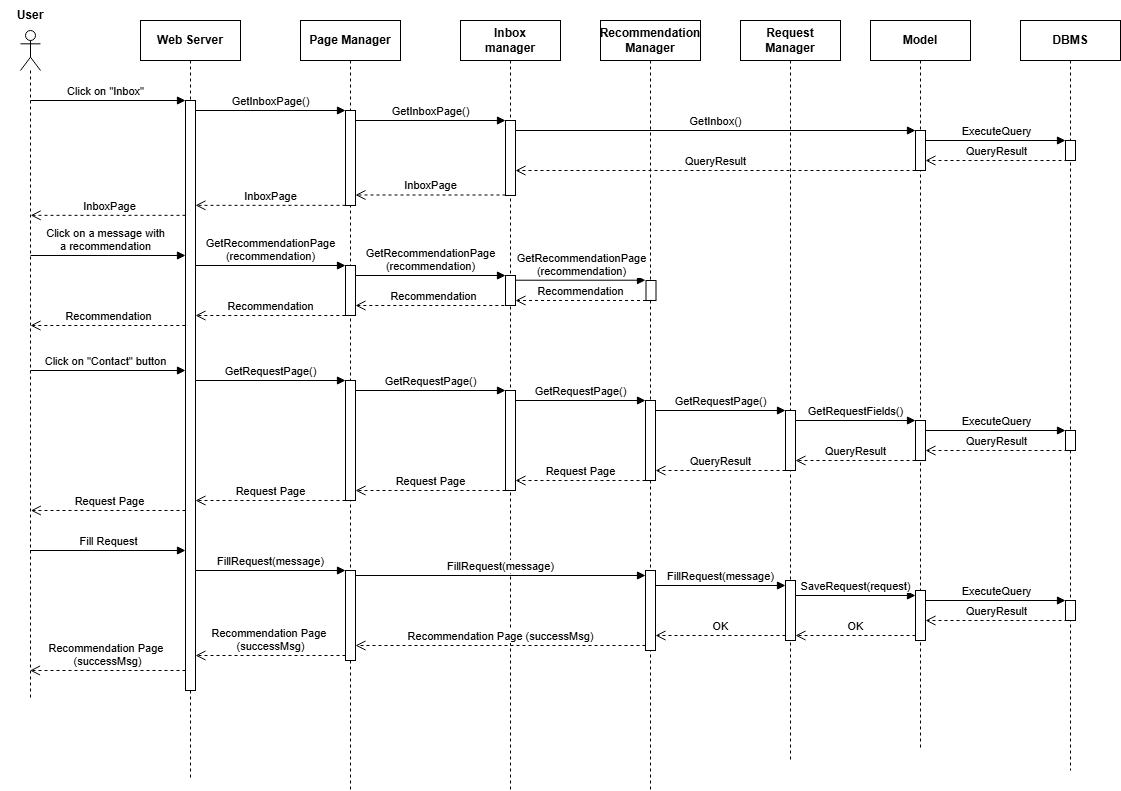
\includegraphics[width=15cm]{images/architectural design/runtime/DD-UC13.drawio.png}
    \caption{SD: Recommendation}
\end{figure}
\textit{Note}: This diagram is generalised for every type of user, so the request's functions are generalised too. The specific ones are used in the search diagrams.

\begin{figure}[H]
\textbf{Accept internship request (Student)}\newline\newline
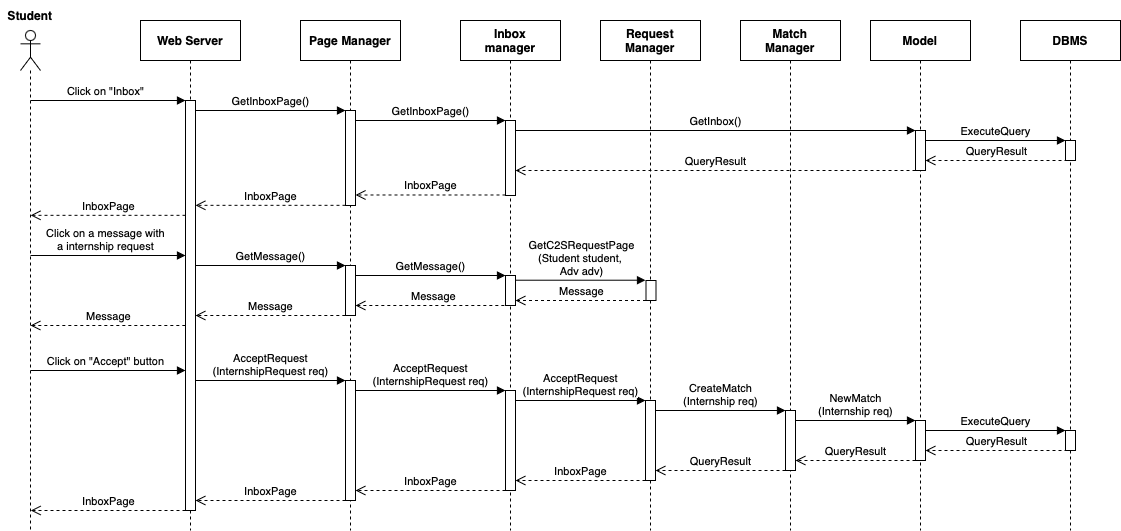
\includegraphics[width=15cm]{images/architectural design/runtime/DD-UC16.1.drawio.png}
    \caption{SD: Accept internship request (Student)}
\end{figure}

\begin{figure}[H]
\textbf{Reject internship request (Student)}\newline\newline
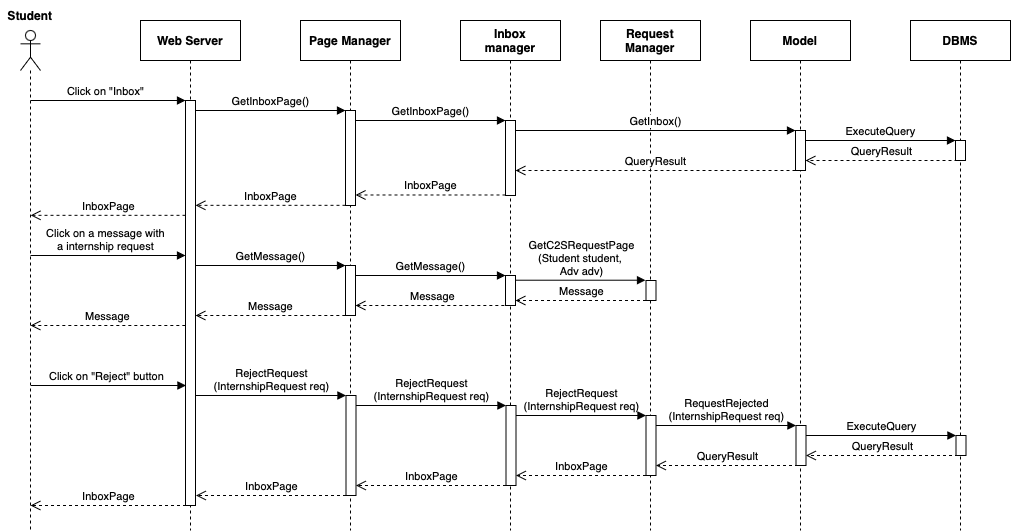
\includegraphics[width=15cm]{images/architectural design/runtime/DD-UC16.2.drawio.png}
    \caption{SD: Reject internship request (Student)}
\end{figure}

\begin{figure}[H]
\textbf{Accept internship request (Company)}\newline\newline
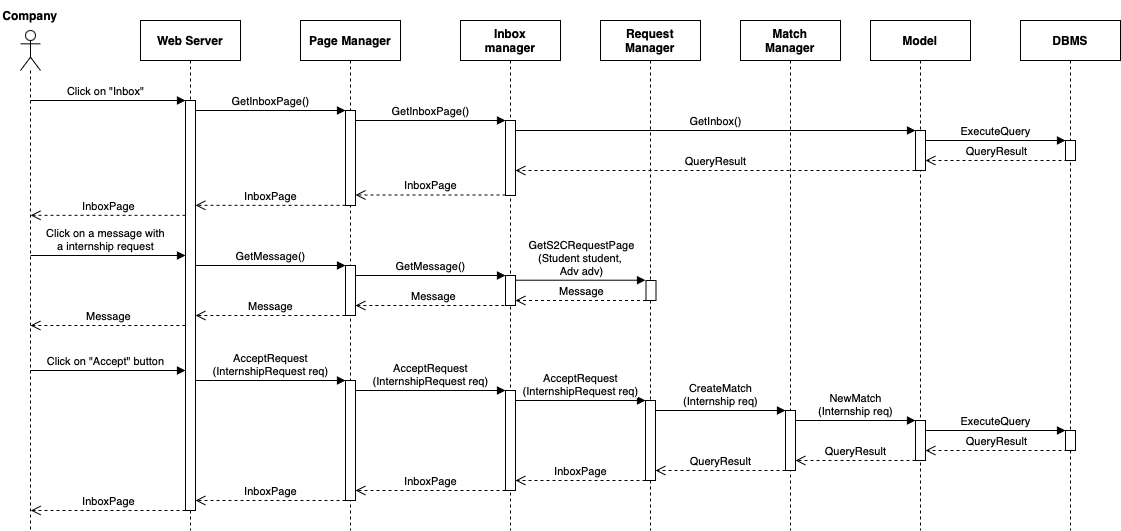
\includegraphics[width=15cm]{images/architectural design/runtime/DD-UC17.1.drawio.png}
    \caption{SD: Accept internship request (Company)}
\end{figure}

\begin{figure}[H]
\textbf{Reject internship request (Company)}\newline\newline
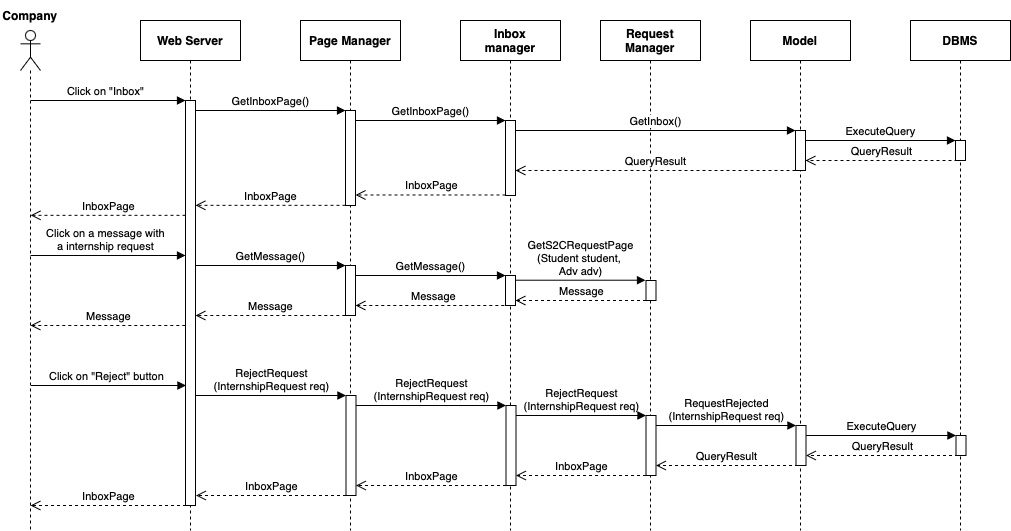
\includegraphics[width=15cm]{images/architectural design/runtime/DD-UC17.2.drawio.png}
    \caption{SD: Reject internship request (Company)}
\end{figure}

\begin{figure}[H]
\textbf{Check request outcome (Student)}\newline\newline
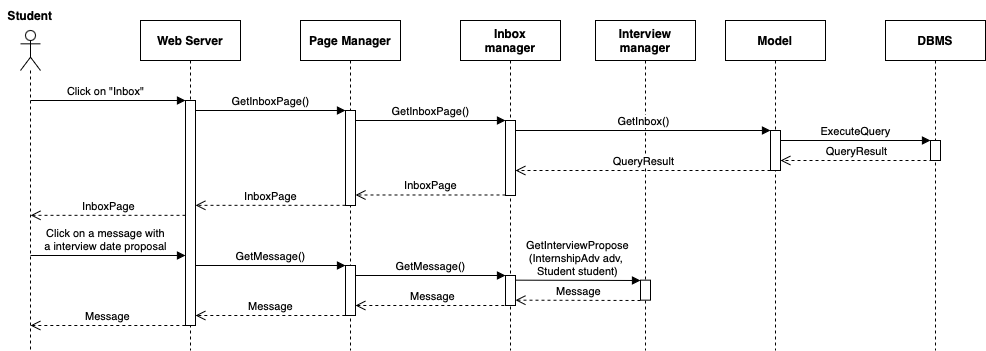
\includegraphics[width=15cm]{images/architectural design/runtime/DD-UC18.drawio.png}
    \caption{SD: Check request outcome (Student)}
\end{figure}

\begin{figure}[H]
\textbf{Check request outcome (Company)}\newline\newline
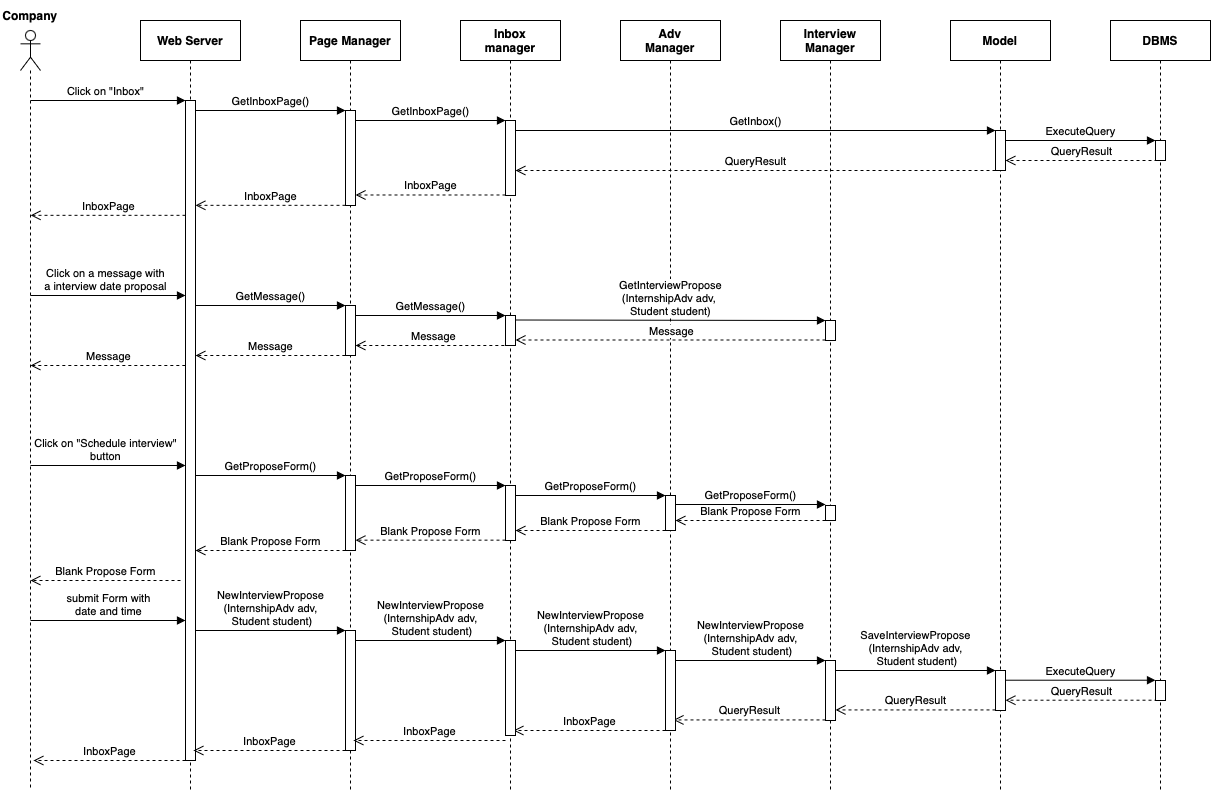
\includegraphics[width=15cm]{images/architectural design/runtime/DD-UC19.drawio.png}
    \caption{SD: Check request outcome (Company)}
\end{figure}

\begin{figure}[H]
\textbf{Propose a date for an interview}\newline\newline
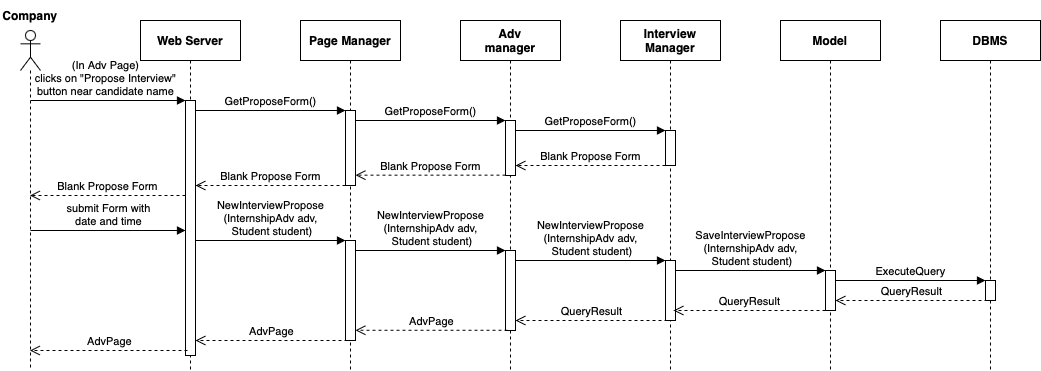
\includegraphics[width=15cm]{images/architectural design/runtime/DD-UC20.1.drawio.png}
    \caption{SD: Propose a date for an interview}
\end{figure}

\begin{figure}[H]
\textbf{Accept a date for an interview}\newline\newline
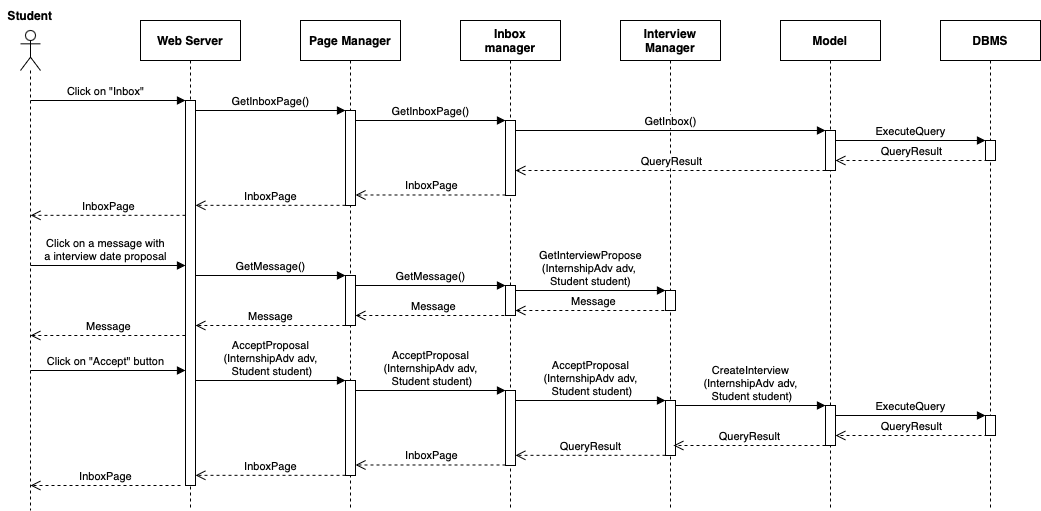
\includegraphics[width=15cm]{images/architectural design/runtime/DD-UC20.2.drawio.png}
    \caption{SD: Accept a date for an interview}
\end{figure}

\begin{figure}[H]
\textbf{Reject a date for an interview}\newline\newline
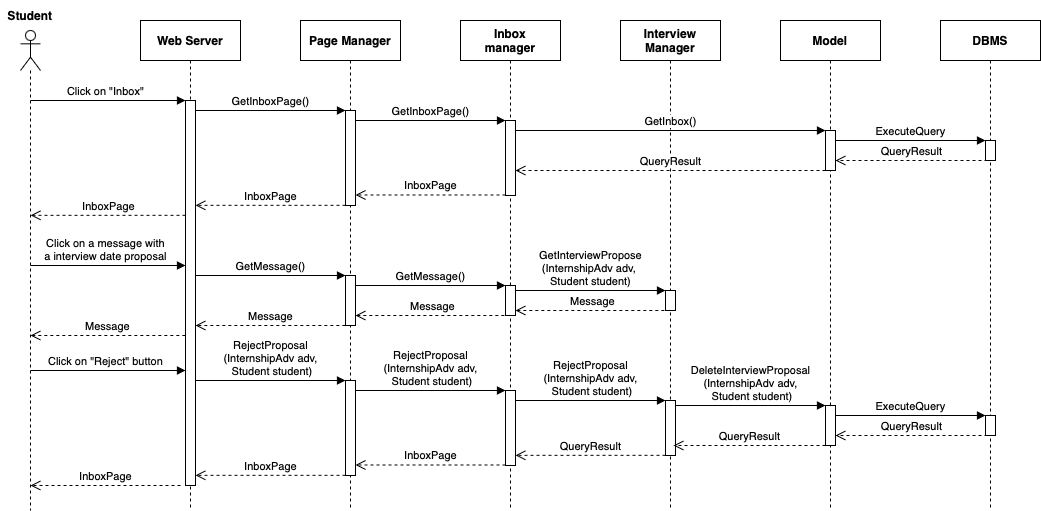
\includegraphics[width=15cm]{images/architectural design/runtime/DD-UC20.3.drawio.png}
    \caption{SD: Reject a date for an interview}
\end{figure}

\begin{figure}[H]
\textbf{Creating form for interview}\newline\newline
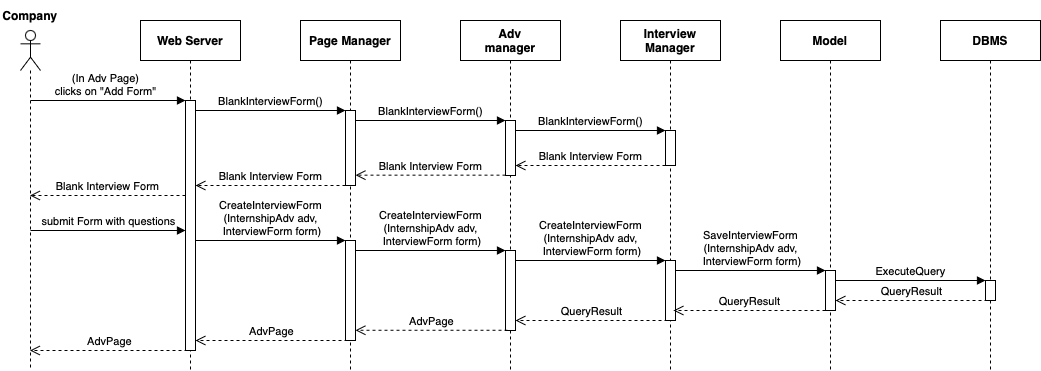
\includegraphics[width=15cm]{images/architectural design/runtime/DD-UC21.drawio.png}
    \caption{SD: Creating form for interview}
\end{figure}

\begin{figure}[H]
\textbf{Deleting form for interview}\newline\newline
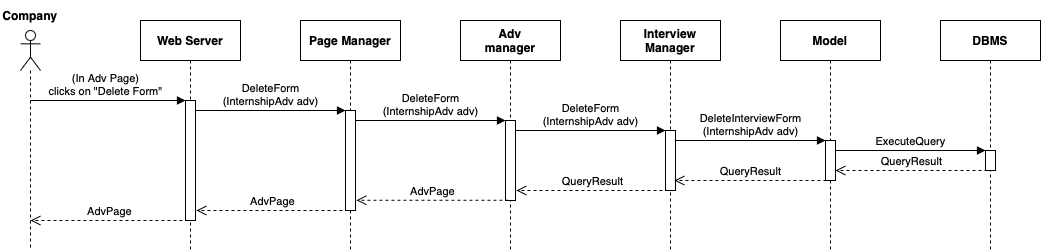
\includegraphics[width=15cm]{images/architectural design/runtime/DD-UC22.1.drawio.png}
    \caption{SD: Deleting form for interview}
\end{figure}

\begin{figure}[H]
\textbf{Modify form for interview}\newline\newline
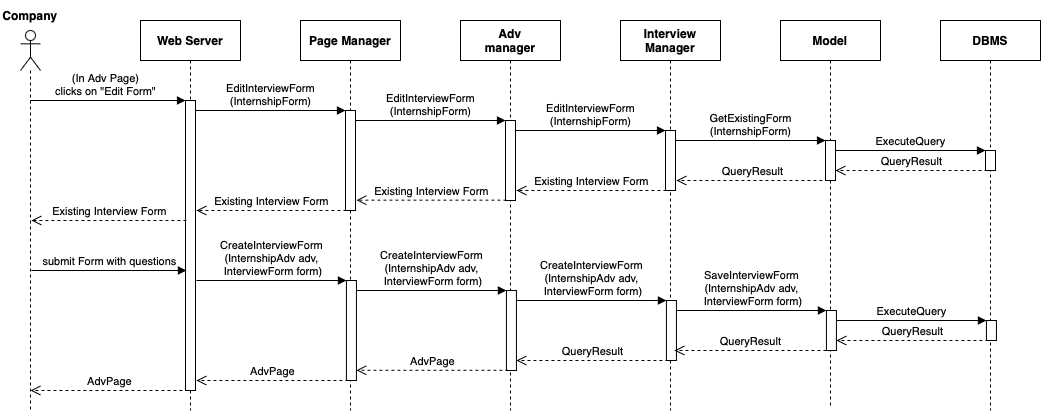
\includegraphics[width=15cm]{images/architectural design/runtime/DD-UC22.2.drawio.png}
    \caption{SD: Modify form for interview}
\end{figure}

\begin{figure}[H]
\textbf{Fill the form during interview}\newline\newline
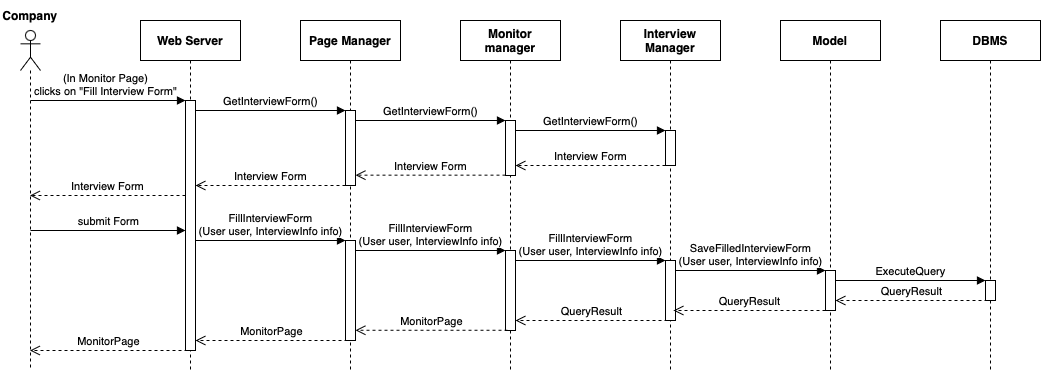
\includegraphics[width=15cm]{images/architectural design/runtime/DD-UC_23.drawio.png}
    \caption{SD: Fill the form during interview}
\end{figure}

\begin{figure}[H]
\textbf{Feedback}\newline\newline
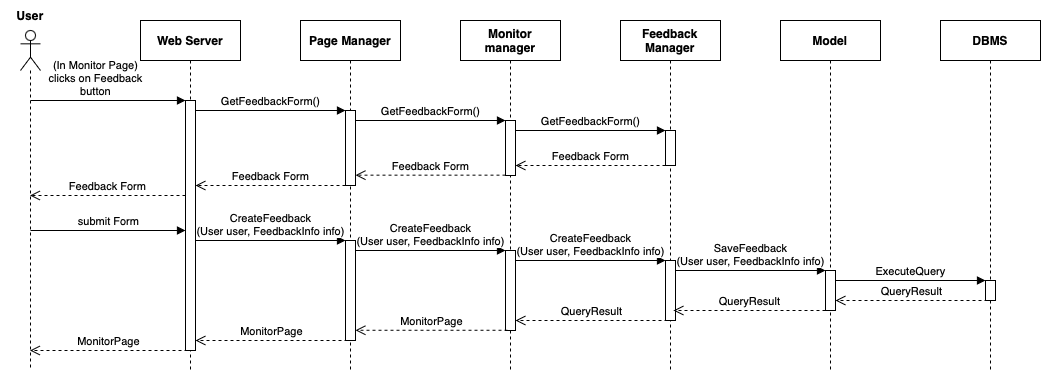
\includegraphics[width=15cm]{images/architectural design/runtime/DD-UC24_25.drawio.png}
    \caption{SD: Feedback}
\end{figure}

\begin{figure}[H]
\textbf{Monitoring}\newline\newline
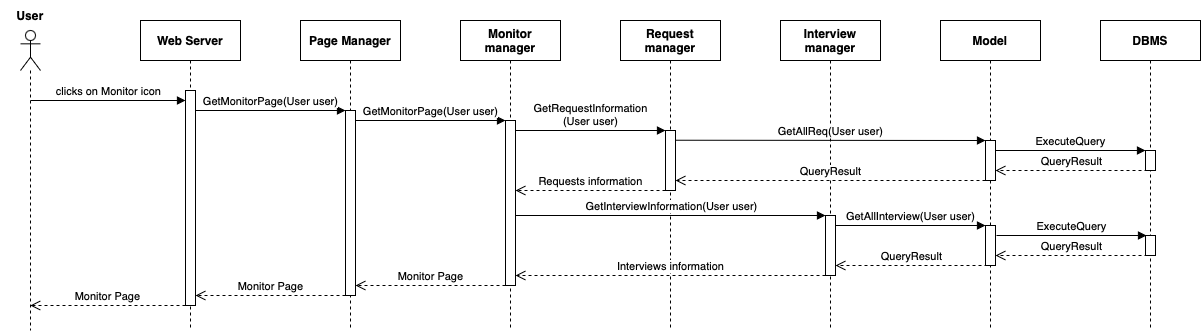
\includegraphics[width=15cm]{images/architectural design/runtime/DD-UC26_27_28.drawio.png}
    \caption{SD: Monitoring}
\end{figure}
\section{Component interfaces}

\begin{itemize}
    \item \textbf{Page Manager}
        \begin{itemize}
            \item It contains all the interfaces of all the others pages
        \end{itemize}
        
    \item \textbf{Registration Manager}
        \begin{itemize}
            \item GetStudentSingupPage()
            \item StudentSingup(String email, String university)
            \item StudentLogin(String email)
            \item GetCompanySingupPage()
            \item CompanySignup(String name, String VAT, File certificate, String email, File authorization)
            \item GetSetPasswordPage()
            \item InsertPassword(String password)
        \end{itemize}
        
    \item \textbf{Login Manager}
        \begin{itemize}
            \item GetStudentLoginPage()
            \item StudentLogin(String email)
            \item GetCompanyLoginPage()
            \item CompanyLogin(String username, String password)
        \end{itemize}
        
    \item \textbf{Request Manager}
        \begin{itemize}
            \item GetS2CRequestPage(Student student, Adv adv)
            \item FillS2CRequest(Student student, Adv adv, String message)
            \item GetC2SRequestPage(Company company, Student student)
            \item FillC2SRequest(Company company, Student student, Adv adv, String message)
            \item GetRequestInformation(User user)
            \item AcceptRequest(InternshipRequest req)
            \item RejectRequest(InternshipRequest req)
        \end{itemize}
        
    \item \textbf{Profile Manager}
        \begin{itemize}
            \item GetProfilePage(User user)
            \item UpdateCV(User user, File pdf)
            \item CheckPdfDimention(File pdf)
            \item AddCompetence(Map<CompetenceEnum, String> competences)
            \item EditCompetence(Competence competence, EnumCompetence type, String description)
        \end{itemize}
        
    \item \textbf{Interview Manager}
        \begin{itemize}
            \item GetInterviewInformation(User user)
            \item GetInterviewForm()
            \item FillInterviewForm(User user, InterviewInfo info)
            \item EditInterviewForm(InternshipForm)
            \item BlankInterviewForm()
            \item CreateInterviewForm(InternshipAdv adv, InterviewForm form)
            \item DeleteForm(InternshipAdv adv)
            \item NewInterviewPropose(InternshipAdv adv, Student student)
            \item GetProposeForm()
            \item GetInterviewPropose(InternshipAdv adv, Student student)
            \item AcceptProposal(InternshipAdv adv, Student student)
            \item RejectProposal(InternshipAdv adv, Student student)
        \end{itemize}
        
    \item \textbf{Adv Manager}
        \begin{itemize}
            \item GetADVsPage(Company company)
            \item GetNewADVForm()
            \item CreateADV(Company company, String name, String location, String profile, String project, String terms)
            \item CheckADV(Adv adv)
            \item GetADVPage(Adv adv)
            \item CreateADV(Company company, String name, String location, String profile, String project, String terms)
            \item EditCompetence(Competence competence, EnumCompetence type, String description)
            \item DeleteADV(Adv adv)
        \end{itemize}
        
    \item \textbf{Inbox Manager}
        \begin{itemize}
            \item GetInboxPage()
        \end{itemize}
        
    \item \textbf{Search Manager}
        \begin{itemize}
            \item GetSearchPage(User user)
            \item InsertInternshipFeatures(User user, List<String> features)
            \item InsertCandidateFeatures(User user, List<String> features)
            \item ElaborateSearchResults(List<Adv> results, List<Match> matches)
        \end{itemize}
        
    \item \textbf{Recommendation Manager}
        \begin{itemize}
            \item GetRecommendationPage(Recommendation recommendation) 
        \end{itemize}
        
    \item \textbf{Match Manager}
        \begin{itemize}
            \item CreateMatch(Internship req)
        \end{itemize}
        
    \item \textbf{Monitor Manager}
        \begin{itemize}
            \item GetMonitorPage(User user)
        \end{itemize}
        
    \item \textbf{Feedback Manager}
        \begin{itemize}
            \item GetFeedbackForm()
            \item CreateFeedback(User user, FeedbackInfo info)
        \end{itemize}
        
    \item \textbf{Model}
         \begin{itemize}
            \item CheckStudent(String email)
            \item CheckUniversity(String university)
            \item CheckCompany(String VAT)
            \item UpdateCompanyInfo(String username, String password)
            \item CheckCompany(String username, String password)
            \item GetUserInfo(User user)
            \item UpdateCV(User user, File pdf)
            \item AddCompetence(Map<CompetenceEnum, String> competences)
            \item EditCompetence(Competence competence, CompetenceEnum type, String description)
            \item GetADVsInfo(Company company)
            \item CreateADV(Company company, String name, String location, String profile, String project, String terms)
            \item GetADVInfo(Adv adv)
            \item EditCompetence(Competence competence, EnumCompetence type, String description)
            \item DeleteADV(Adv adv)
            \item GetUserSuggestedSearch(User user)
            \item GetSearchResult(List<String> features)
            \item GetStudentMatches(Student student)
            \item GetCompanyInfo(Adv adv)
            \item SaveS2CRequest(Student student, Adv adv, String message)
            \item SaveC2SRequest(Company company, Student student, Adv adv, String message)
            \item GetCompanyMatches(Company company)
            \item SaveSearchFields(Student student, List<String> fields)
            \item GetAllInterview(User user)
            \item GetAllReq(User user)
            \item SaveFeedback(User user, FeedbackInfo info)
            \item SaveInterviewForm(InternshipAdv adv, InterviewForm form)
            \item GetExistingForm(InternshipForm)
            \item SaveFilledInterviewForm(User user, InterviewInfo info)
            \item DeleteInterviewForm(InternshipAdv adv)
            \item GetInbox
            \item SaveInterviewPropose(InternshipAdv adv, Student student)
            \item DeleteInterviewProposal(InternshipAdv adv, Student student)
            \item NewMatch(Internship req)
            \item RequestRejected(InternshipRequest req)
        \end{itemize}   
\end{itemize}

\section{Selected architectural styles and patterns}
\label{subsec: 2.6 Selected architectural styles and patterns}
The S\&C system uses a combination of architectural styles and design patterns to ensure modularity, scalability, and maintainability. The core of the system is built around \textbf{Micro-service Architecture} and is integrated with a \textbf{3-Tier Architecture} and a \textbf{Client-Server Model}. These enable the system to meet performance and goals while maintaining flexibility.
\subsection{Micro-service Architecture}
The Micro-service Architecture divides the application into independent service, each one responsible for a specific functionality. It enables efficient development, testing, deployment, and scaling thanks to its modularity, each micro-service operates independently, communicating with other through APIs. A unified \textbf{API Gateway} serves as a centralised entry point for client requests, reducing direct interactions between clients and individual micro-services.
\subsection{3-Tier Architecture}
The 3-Tier Architecture is a software design model that organises the application into three layers. This model ensures modularity (each tier can be developed individually), scalability, maintainability (the separation of concerns allows for easier debugging), and security (it isolates the data, so the direct access to it is restricted). The three layers are:
\begin{enumerate}
    \item \textbf{Presentation Tier}, i.e. the user interface layer: this tier displays information to users and collects their input. In the S\&C platform, it is represented by the web pages and is located on the Web Server node of the physical architecture. This layer interacts with the micro-service through the unified API Gateway.
    \item \textbf{Application Tier}, i.e. the business logic layer: This tier contains the function to process input, execute decisions, and perform computations. It works as a bridge between the first and third layers. In the S\&C system is represented through the Model and is placed on the Application Server node. It ensures efficient data processing and coordination among micro-services.
    \item \textbf{Data Tier}: this tier stores and manages data through databases.
\end{enumerate}
\subsection{Client-Server Model}
The communication framework is developed following the Client-Server Model. The client is the web browser, it sends requests to the server using HTTPS protocol. The server processes the client's requests and provides responses. The Presentation Tier formats the server's responses while the Application Tier processes the client's requests.

\section{Other design decisions}
\subsection{Scalability}
The micro-services architecture implementation, as opposite at the monolithic one, enable a fine-gained scaling strategies, allowing a flexible deployment and more over a selective replication. Accordingly, with this approach we are able to scale the individual components rather than the entire system.

\subsection{Ease of Deployment}
The micro-services approach allows to enhance the ease of deployment, working with many smaller components, rather that a single big one, we can easily update them, test them and deploy them independently and, more over we can update and deploy the single components in parallel. Furthermore, with this approach we reduce the risks of critical errors, which can also be repaired easily in case they occur.

\pagebreak
\chapter{User Interface Design}
\section{Overview}
\begin{figure}[H]
    \centering
    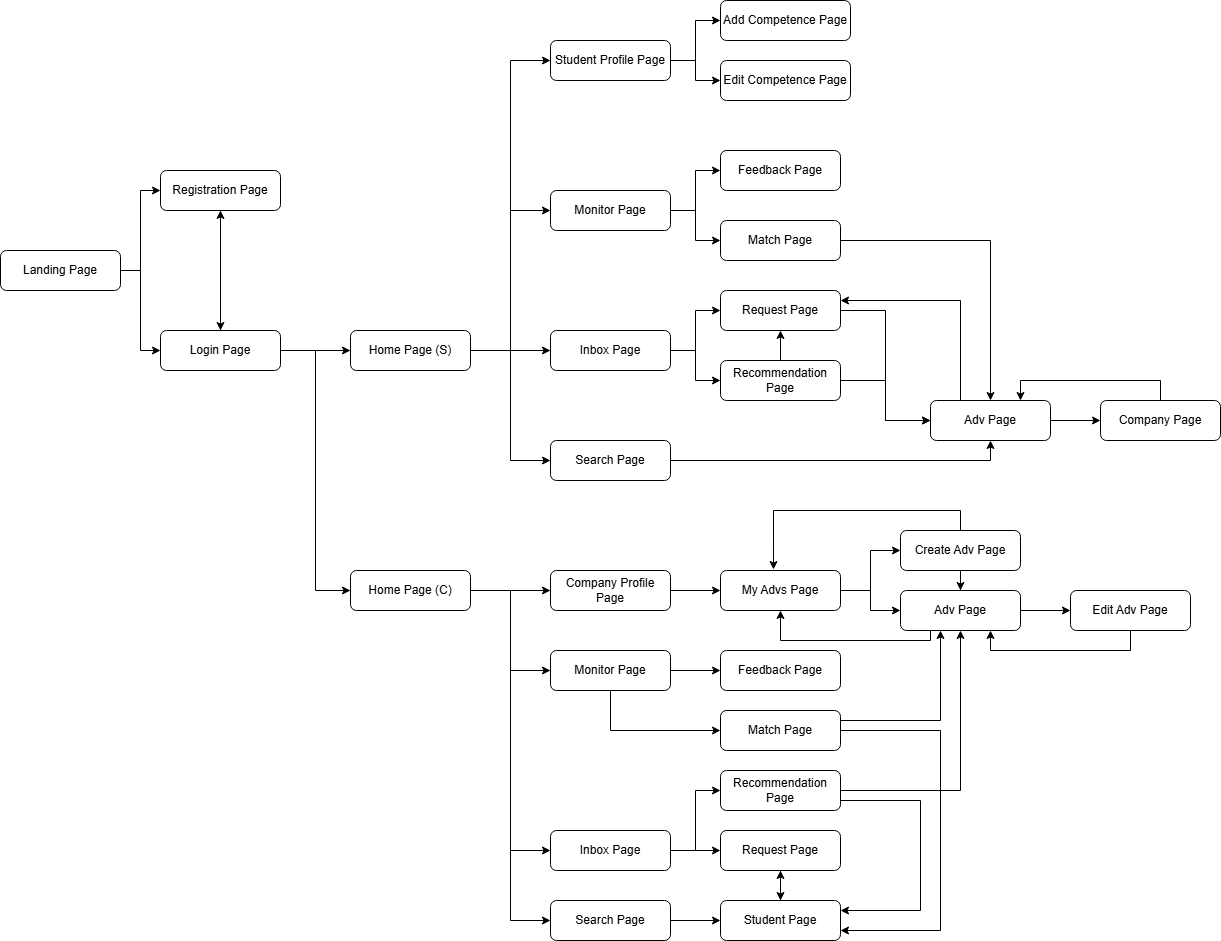
\includegraphics[width=15cm]{images/ui/DD-UI-Overview.drawio.png}
    \caption{User Interface Overview}
\end{figure}
This diagram shows how users can navigate the platform. Upon entering the website's URL, they are directed to the \textbf{Landing Page}, where they can choose between Registration and Login. Both pages allow users to switch to the other if needed. After logging in, users are redirected to their personalised \textbf{Home Page}, which varies depending on their role (S - Student, C - Company). A navigation bar is present on all pages, enabling users to move across the most relevant sections, i.e. \textbf{Profile Page}, \textbf{Monitor Page}, \textbf{Inbox Page}, and \textbf{Search Page}. The arrows in the diagram represent links between pages, but not all links are shown to maintain diagram clarity. Additionally, back buttons are available on each page to facilitate navigation.
When a student visits an \textbf{ADV Page}, they can send a request regarding that ADV (as shown by the arrow linking the Adv Page to the Request Page). Similarly, companies can perform the same action when viewing a student’s profile page.
Lastly, as discussed in the RASD document, users can provide feedback via the \textbf{Monitor Page}.
\section{Mock-up pages}
\subsection{Login Page}
\begin{figure}[H]
    \centering
    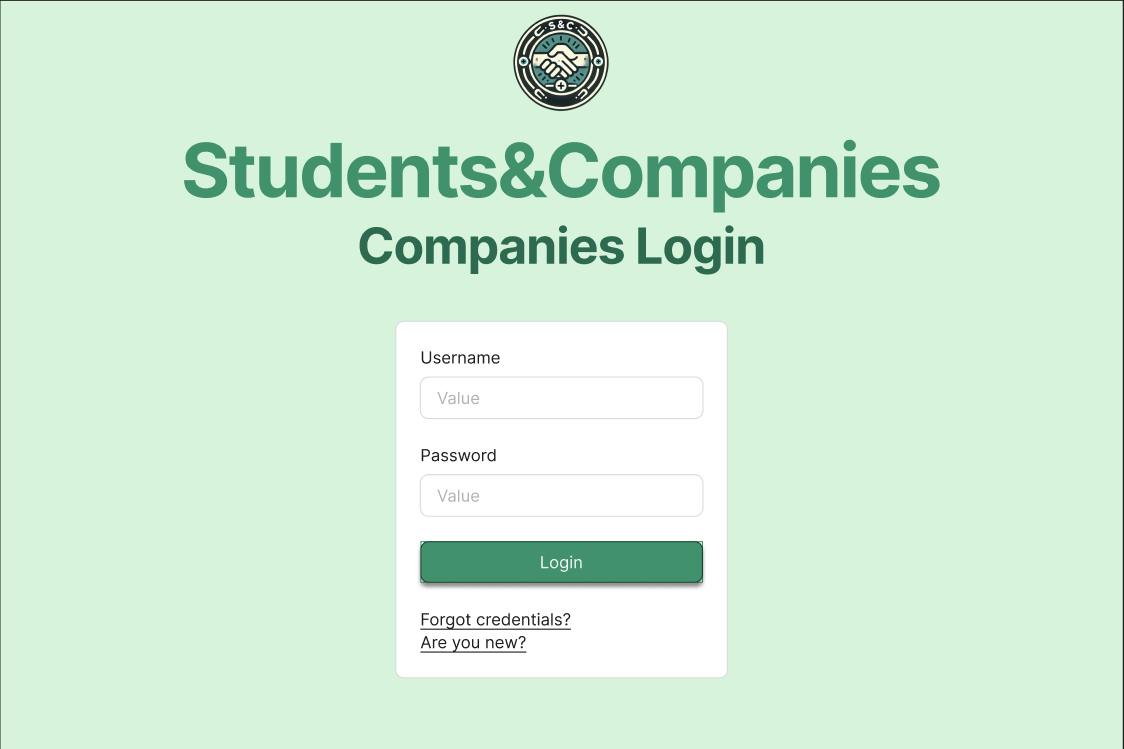
\includegraphics[width=15cm]{images/ui/login.jpg}
    \caption{UI: Login Page}
\end{figure}
This is the Login Page for companies. As precedent discussed, the company's representative can insert the username and the password given at the moment of registration. If they do not remember the password or the username, they can click on the "Forgot credentials?" link, they will have to insert their company email and they will be able to reset the credentials. If the company is not registered, the representative can click on the "Are you new?" link to be redirected to the Sign up Page.

The student's login page is not shown because similar.

\subsection{Sign Up Page}
\begin{figure}[H]
    \centering
    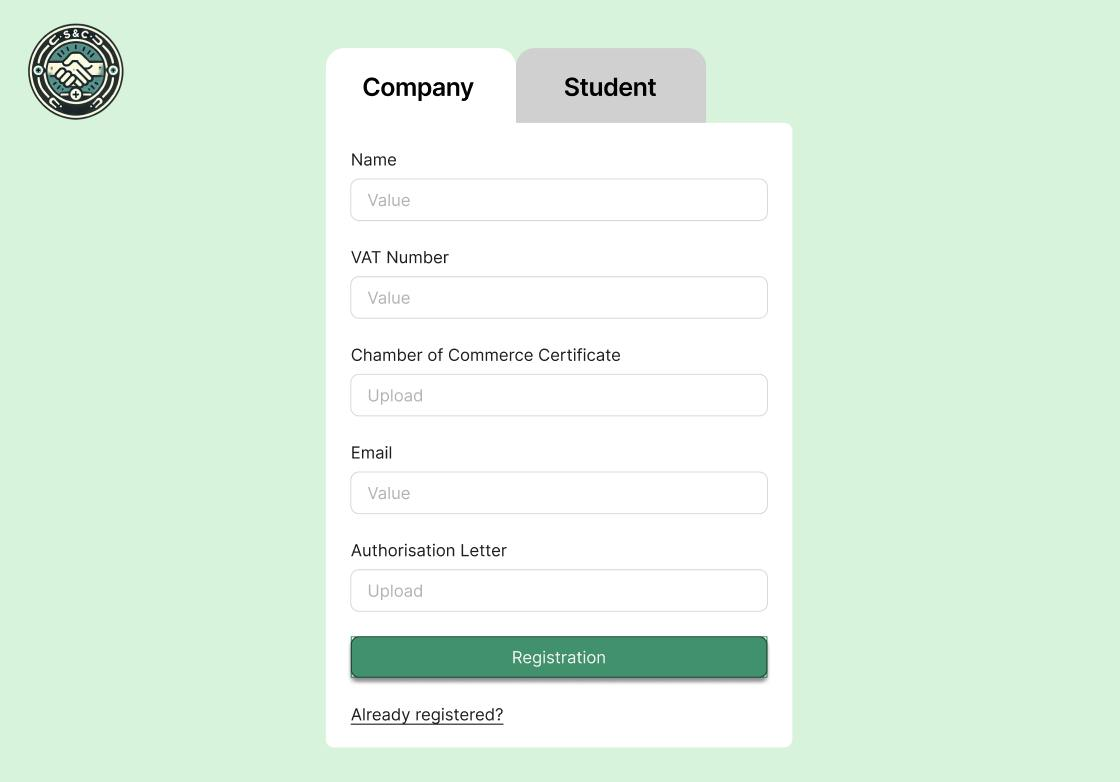
\includegraphics[width=15cm]{images/ui/signup.jpg}
    \caption{UI: Sign up Page}
\end{figure}
This is the form shown to companies that want to register to the platform. If someone is already registered, they can click on the "Already registered?" link and will be redirected to the Login Page. Students can click on the "Student" section to compile their form. This is not shown because is similar.

\subsection{Home Page}
\begin{figure}[H]
    \centering
    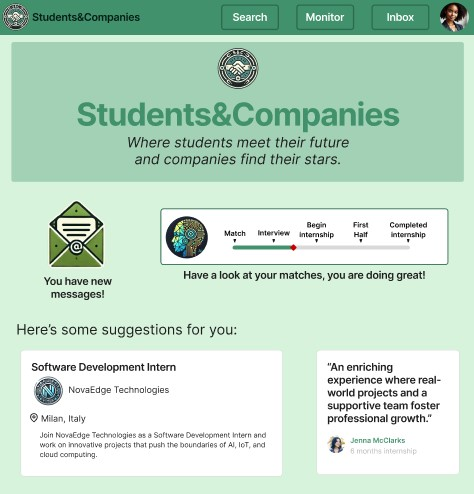
\includegraphics[width=15cm]{images/ui/homepage.jpg}
    \caption{UI: Home Page}
\end{figure}
The \textbf{navigation bar} contains the logo and the name of the platform, they are clickable and directs to the Home Page. The other buttons direct to the correspondent pages, and the profile picture directs to the profile.
The home page is personalised: in this case there is the envelope image that directs the user to the Inbox Page, and the monitor bar that redirects to the Monitor Page. The suggestions are linked to the Company Profile and to the ADV.

\subsection{Student Profile Page}
\begin{figure}[H]
    \centering
    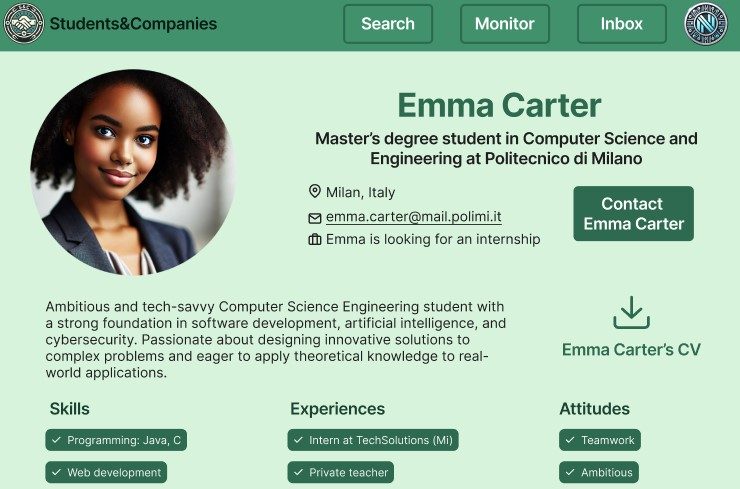
\includegraphics[width=15cm]{images/ui/studentprofile.jpg}
    \caption{UI: Student Profile Page}
\end{figure}
This is a student's Profile Page seen by a company. By clicking on the download icon or on the "Emma Carter's CV" link, a user can download the student's CV. By clicking on one of the shown competence, a pop-up window opens and shows the description inserted by the student. If a company is interested, they can click on the "Contact Emma Carter" button to send an Internship Request to the student. By scrolling the page all the competences are show, as well as relevant comments left by the companies.
\begin{figure}[H]
    \centering
    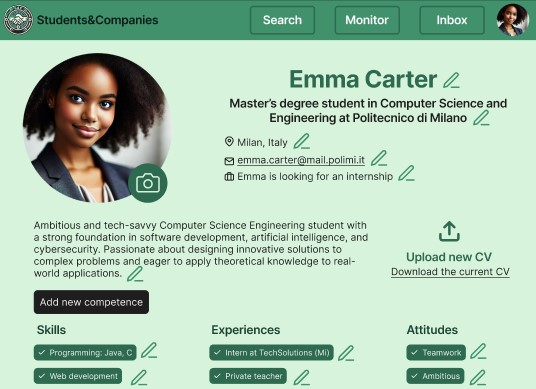
\includegraphics[width=15cm]{images/ui/studentprofilepersonal.jpg}
    \caption{UI: Student Personal Profile Page}
\end{figure}
This image shows how the student sees their own personal page. They can modify all the information by clicking on the pen icon, they can upload a new profile image by clicking on the camera icon, they can upload a new CV by clicking on the upload icon but also they can download the current one, and they can add a new competence by clicking on the button.

\subsection{Company Profile Page}
\begin{figure}[H]
    \centering
    \includegraphics[width=15cm]{images/ui/companyprofile.jpg}
    \caption{UI: Company Profile Page}
\end{figure}
This is a company's profile seen by students. All the company's active ADVs are shown in the boxes on the left, they are clickable and bring the user to the ADV page. On the right, relevant comments by students are shown.

\subsection{Company's ADVs Page}
\begin{figure}[H]
    \centering
    \includegraphics[width=15cm]{images/ui/advspage.jpg}
    \caption{UI: Company's ADVs Page}
\end{figure}
When a Company is logged in, the representative can reach the ADVs Page from the personal profile. A new ADV can be created by clicking on the button, and the other ones can be modified by clicking on the corresponding "Edit" button. ADVs can be found via the search bar and/or applying filters. The Interview Form can be created by clicking on the "Edit" button.

\subsection{Company's ADV Page}
\begin{figure}[H]
    \centering
    \includegraphics[width=15cm]{images/ui/advpage(1).png}
    \caption{UI: Company's ADV Page}
\end{figure}
When a Company is logged in, the representative can visualize ADV Page from the personal profile. The ADV can be edited by clicking on the "Edit" button, the representative can add a form to help the evaluation of the candidates during the interview by clicking on "+ Interview Form", or can delete the advertisement by clinking on "Delete" button. From this page the representative can also see all the students that has done a match with this Adv and setting up an interview with them pressing on "Propose Interview" button near the candidate name.


\subsection{ADV Page}
\begin{figure}[H]
    \centering
    \includegraphics[width=15cm]{images/ui/advpage.jpg}
    \caption{UI: ADV Page}
\end{figure}
This is the ADV Page seen by students. It contains all the information about the Internship position (all viewable by scrolling the page). By clicking on the company's logo or the name, the student is redirected to the company's profile. A student can contact the company regarding this ADV by clicking on the "Contact" button. On the left links to similar offers are shown.

\subsection{Search Page}
\begin{figure}[H]
    \centering
    \includegraphics[width=15cm]{images/ui/search.jpg}
    \caption{UI: Search Page}
\end{figure}
The Search Page contains a search bar where the user (in this case a student) can insert key words. The user can also use the filters on the left or try the suggested key words on the right. When clicking on the "View ADV" button the student is redirected to the ADV page, while by clicking on the company's name they are redirected to the company's profile.

\subsection{Monitor Page}
\begin{figure}[H]
    \centering
    \includegraphics[width=15cm]{images/ui/monitor.jpg}
    \caption{UI: Monitor Page}
\end{figure}
The Monitor Page contains the match done, in this case it contains the ADV with which the student matched. For each ADV the student can see the progress and click on the "Feedback" button to leave one.
The companies Monitor Page first has the list of the ADVs, when clicking on one of them the company is redirected to the monitor page of that ADV so they will see a list of student that have match with that adv, just as the image above.

\subsection{Inbox Page}
\begin{figure}[H]
    \centering
    \includegraphics[width=15cm]{images/ui/inbox.jpg}
    \caption{UI: Inbox Page}
\end{figure}
This is the Inbox Page, it works as a standard mail box. 

\pagebreak
\chapter{Requirements Traceability}
\begin{itemize}
    \item \textbf{Registration Manager}
        \begin{itemize}
            \item[\text{[R1]}] S\&C allows Students to sign up to the platform through their university credentials using SSO access.
            \item[\text{[R3]}] S\&C allows Companies to sign up to the platform by asking the representative of the company to insert their company email, the VAT number of the company, a Certificate of registration at the Chamber of Commerce, and a letter of authorisation or official assignment signed by a CEO or a HR referent. They have to choose a password.
        \end{itemize}
        
    \item \textbf{Login Manager}
        \begin{itemize}
            \item[\text{[R2]}] S\&C allows Student to login via their university credentials.
            \item[\text{[R4]}] S\&C allows Companies to login to the platform via password and username (created by the system).
        \end{itemize}

        \item \textbf{Profile Manager}
        \begin{itemize}
            \item[\text{[R5]}] S\&C allows Students to upload the PDF of their CV (both for the first time and other times if there have been some changes).
            \item[\text{[R6]}] S\&C allows Students to insert new experiences, skills, and attitudes on their profile.
            \item[\text{[R7]}] S\&C allows Students to edit or delete experiences, skills, and attitudes present on their profile.
        \end{itemize}

        \item \textbf{Adv Manager}
        \begin{itemize}
            \item[\text{[R8]}] S\&C allows Companies to create an advertisement regarding an internship position they are offering, explaining the project of the internship and the terms offered.
            \item[\text{[R9]}] S\&C allows Companies to modify and remove an advertisement posted on their page.
        \end{itemize}

        \item \textbf{Search Manager}
        \begin{itemize}
            \item[\text{[R10]}] S\&C allows Students to use a research bar to find appropriate internship positions by inserting specific requirements about the project and/or the terms offered.
            \item[\text{[R11]}] S\&C allows Companies to use a research bar to find appropriate candidates for their internship positions by inserting specific experiences, skills and/or attitudes the candidates should have.
        \end{itemize}

        \item \textbf{Recommendation Manager}
        \begin{itemize}
            \item [\text{[R12]}] S\&C informs students when an internship that might interest them becomes available.
            \item [\text{[R13]}] S\&C informs companies about the availability of a student whose CV corresponds to their needs. 
        \end{itemize}
        
    \item \textbf{Request Manager}
        \begin{itemize}
            \item [\text{[R14]}] S\&C allows Students to contact a company they are interested in.
            \item [\text{[R15]}] S\&C allows Companies to contact Students they are interested in.
            
        \end{itemize}

        \item \textbf{Inbox Manager}
        \begin{itemize}
            \item [\text{[R16]}] S\&C informs a Student when a Company shows interest in their profile by sending the Student the Company's offer. The Student can accept or decline the offer.
            \item [\text{[R17]}] S\&C informs a Company when a Student shows interest in its offer by sending to the Company the Student's CV, the Company can accept or decline the offer.
            \item [\text{[R18]}] S\&C communicates to Students or Companies if their requests are successful.
        \end{itemize}

        \item \textbf{Match Manager}
        \begin{itemize}
            \item [\text{[R18]}] S\&C communicates to Students or Companies if their requests are successful.
            \item [\text{[R19]}] S\&C allows Companies to setup an interview with the candidates.
        \end{itemize}
        
    \item \textbf{Interview Manager}
        \begin{itemize}
            \item [\text{[R19]}] S\&C allows Companies to setup an interview with the candidates.
            \item [\text{[R20]}] S\&C allows Companies to write a form with all the aspects that will be considered during the interviews.
            \item [\text{[R21]}] S\&C allows Companies to modify or delete the interview form created.
            \item [\text{[R22]}] S\&C allows Companies fill the form during the interview.
        \end{itemize}

        \item \textbf{Feedback Manager}
        \begin{itemize}
            \item [\text{[R23]}] S\&C allows Students to give personal feedback during the selection period about the Company's selection method or during the internship period about the internship itself.
            \item [\text{[R24]}] S\&C allows Companies to give feedback after the interview or during the internship about a single Student.
        \end{itemize}

        \item \textbf{Monitor Manager}
        \begin{itemize}
            \item [\text{[R25]}] S\&C offers Students the possibility to monitor their matchmaking process with a Company (state of the matchmaking, scheduled interview, interview results).
            \item [\text{[R26]}] S\&C offers Companies the possibility to monitor their matchmaking process with a Student.
            \item [\text{[R27]}] S\&C offers Students and Companies the possibility to monitor the state of the internship.
        \end{itemize}
\end{itemize}


\pagebreak
\chapter{Implementation, Integration and Test Plan}
\section{Overview and Implementation Plan}
The Implementation, Integration and Test phases will follow a \textbf{Bottom-Up} strategy. This approach consists in develop and evaluate the components individually, and then integrate them into a larger system. Working with micro-services, this strategy will be followed starting from the low level components (model, login, and registration) and then continuing building the entire ecosystem around them. At each step some driver will be created in order to test the components. This strategy will allow developers to keep tracks of eventual bugs or errors, and furthermore will allow a parallel developing workflow.

\section{Integration Strategy}
The implementation will be executed in a bottom-up way, starting from the basic feature and component, and after them, with their related test, the above components will be implemented.

\begin{figure}[H]
The implementation starts with the model component and its test.
    \begin{center}
        \includegraphics[width=3cm]{images/IntegrationStrategy/model.png}
        \caption{Model implementation}
    \end{center}
\end{figure}

\begin{figure}[H]
The implementation continues with the Login and Signup components, with a particular attention to the university and the Revenue Agency API interaction. At the same time the creation of an Adv of an internship and the Update of a profile can be implemented.\newline
    \begin{center}
        \includegraphics[width=10cm]{images/IntegrationStrategy/login_signup_adv_update.png}
        \caption{Login, Signup, creation of an adv and the update of a profile implementation}
    \end{center}
\end{figure}

\begin{figure}[H]
After Adv creation, Proactive research and Recommendation can be implemented, as long as the creation of the Interview form.\newline
    \begin{center}
        \includegraphics[width=10cm]{images/IntegrationStrategy/proac_recom_intForm.png}
        \caption{Proactive Research, Recommendation and interview form implementation}
    \end{center}
\end{figure}

\begin{figure}[H]
The implementation continues with the Request component, which is directly linked to the Recommendation and to the Proactive Research.
    \begin{center}
        \includegraphics[width=8cm]{images/IntegrationStrategy/req.png}
        \caption{Request implementation}
    \end{center}
\end{figure}

\begin{figure}[H]
After Request implementation, the Match component can be implemented.\newline
    \begin{center}
        \includegraphics[width=8cm]{images/IntegrationStrategy/match.png}
        \caption{Match and Feedback implementation}
    \end{center}
\end{figure}

\begin{figure}[H]
Then the Interview i implemented and at the same time the Feedback section can be implemented and, during these finals implementation, the system can be joined in order test it in its entirety.
    \begin{center}
        \includegraphics[width=15cm]{images/IntegrationStrategy/interview_feedback.png}
        \caption{Interview and Feedback implementation and join all the system}
    \end{center}
\end{figure}

\begin{figure}[H]
The latter implementation section will involve the Page Manager and all the pages of the Application.
    \begin{center}
        \includegraphics[width=15cm]{images/IntegrationStrategy/page_manager.png}
    \caption{View implementation}
    \end{center}
\end{figure}

\section{System Testing Strategy}
Following the Bottom-Up strategy, every component will be tested with a Driver during the implementation phase but also during the integration phase, in order to assure its functionality independently but also its communication features with all the other components of the system. The test that will be performed are:
\begin{itemize}
    \item \textbf{Functional test:}
    This test sections will ensure that every components fulfill the designated job, accordingly with the system goals, requirement and functionality of the system.
    \item \textbf{Performance test:}
    This type of test are designated to finds bottlenecks and identify some critical situation that may occur during an heavy workload periods. This tests are also useful to get some idea of possible future update and enhancements.
    \item \textbf{Load test:}
    This type of test will cover the discover of memory problems such as leak or overflows.
    \item \textbf{UI test:}
    This type of test will evaluate the Usability of the System for all the users, and will establish if the System works on different type of browser.
\end{itemize}

\pagebreak
\chapter{Effort Spent}
This is an overview of the number of hours spent on each chapter. Most of the work was done in pairs. However, an approximation of the number of hours contributed by each member is provided.
\begin{table}[]
    \centering
    \begin{tabular}{|c|c|c|}
        \hline
        - & \textbf{Irene Lo Presti} & \textbf{Matteo Lussana} \\\hline
        Introduction & 2h & 0.5h \\\hline
        Architectural Design & 18h & 17h \\\hline
        User Interface Design & 15h & 13h \\\hline
        Requirements Tracebility & 0.5h & 0.5h \\\hline
        Implementation, Integration, and Test Plan & 0.5h & 3h \\\hline
    \end{tabular}
\end{table}

\pagebreak
\chapter{References}
\section{References}
\begin{itemize}
    \item Specification document: Assignment RDD AY 2024-2025. 
    \item Slides of the course "Software Engineering 2" held at Politecnico di Milano by Professor Rossi (a.y. 2024-25).
    \item Some definitions from the Definitions, Acronyms, Abbreviations section are taken from researches done on the Internet.
\end{itemize}
\section{Used Tools}
\begin{itemize}
    \item GitHub for project versioning and sharing.
    \item \LaTeX\space and \textit{Overleaf} as editor for writing this document.
    \item \textit{draw.io} for diagrams design.
    \item \textit{Notion} for collaborative organisation.
\end{itemize}

\pagebreak
\listoffigures




\end{document}
